%%%%%%%%%%%%%%%%%%%%%%%%%%%%%%%%%%%%%%%%%
% Journal Article
% LaTeX Template
% Version 1.3 (9/9/13)
%
% This template has been downloaded from:
% http://www.LaTeXTemplates.com
%
% Original author:
% Frits Wenneker (http://www.howtotex.com)
%
% License:
% CC BY-NC-SA 3.0 (http://creativecommons.org/licenses/by-nc-sa/3.0/)
%
%%%%%%%%%%%%%%%%%%%%%%%%%%%%%%%%%%%%%%%%%

%----------------------------------------------------------------------------------------
%	PACKAGES AND OTHER DOCUMENT CONFIGURATIONS
%----------------------------------------------------------------------------------------

\documentclass[a4paper, 12pt, twoside]{article}

\usepackage{lipsum} % Package to generate dummy text throughout this template
\usepackage[utf8x]{inputenc}
\usepackage[T1]{fontenc}
\PrerenderUnicode{áéíóúñ}
%\usepackage[spanish]{babel}
%\usepackage{t1enc}
\usepackage[english]{babel}
\usepackage{pdfpages}
\usepackage{graphicx}
\usepackage{sidecap}
\usepackage{amssymb,amsmath}
\usepackage{mathtools}
\usepackage{amsmath}
\usepackage{mathrsfs}
\usepackage{wrapfig}
\usepackage{float}
\usepackage[firstpage]{draftwatermark}
\usepackage[sc]{mathpazo} % Use the Palatino font
\usepackage[T1]{fontenc} % Use 8-bit encoding that has 256 glyphs
\linespread{1.05} % Line spacing - Palatino needs more space between lines
\usepackage{microtype} % Slightly tweak font spacing for aesthetics
\usepackage{url}
\usepackage[hmarginratio=1:1,top=25mm,columnsep=25pt,left=25mm]{geometry} % Document margins
\usepackage{multicol} % Used for the two-column layout of the document
\usepackage{color}
\usepackage[hang, small,labelfont=bf,up,textfont=it,up]{caption} % Custom captions under/above floats in tables or figures
\usepackage{booktabs} % Horizontal rules in tables
\usepackage{float} % Required for tables and figures in the multi-column environment - they need to be placed in specific locations with the [H] (e.g. \begin{table}[H])
\usepackage{hyperref} % For hyperlinks in the PDF
\usepackage{caption}
\usepackage{lettrine} % The lettrine is the first enlarged letter at the beginning of the text
\usepackage{paralist} % Used for the compactitem environment which makes bullet points with less space between them
\def\textsubscript#1{\ensuremath{_{\mbox{\textscale{.6}{#1}}}}}
\usepackage{abstract} % Allows abstract customization
\renewcommand{\abstractnamefont}{\normalfont\bfseries} % Set the "Abstract" text to bold
\renewcommand{\abstracttextfont}{\normalfont\small\itshape} % Set the abstract itself to small italic text
\usepackage{titlesec} % Allows customization of titles
\graphicspath{ {pics/} }
\titleformat{\section}[block]{\large\scshape\centering}{\thesection.}{1em}{} % Change the look of the section titles
\titleformat{\subsection}[block]{\large\bf}{\thesubsection.}{1em}{} % Change the look of the section titles
\titleformat{\subsubsection}[block]{\large}{\thesubsubsection.}{1em}{} % Change the look of the section titles
\renewcommand{\labelitemi}{$\bullet$}
\renewcommand{\labelitemii}{$\cdot$}
\renewcommand{\labelitemiii}{$\diamond$}
\renewcommand{\labelitemiv}{$\ast$}
\newcommand{\myparagraph}[1]{\paragraph{#1}\mbox{}\\}
\setcounter{secnumdepth}{5}
\setcounter{tocdepth}{5}


\usepackage{fancyhdr} % Headers and footers
\pagestyle{fancy} % All pages have headers and footers
%\fancyhead{} % Blank out the default header
%\fancyfoot{} % Blank out the default footer
%\fancyhead[C]{Metallicity Gradients in ies $\bullet$ December 2015} % Custom header text

%\fancyfoot[RO,LE]{\thepage} % Custom footer text
%----------------------------------------------------------------------------------------
%	TITLE SECTION
%----------------------------------------------------------------------------------------

\SetWatermarkLightness{0.2}
\SetWatermarkText{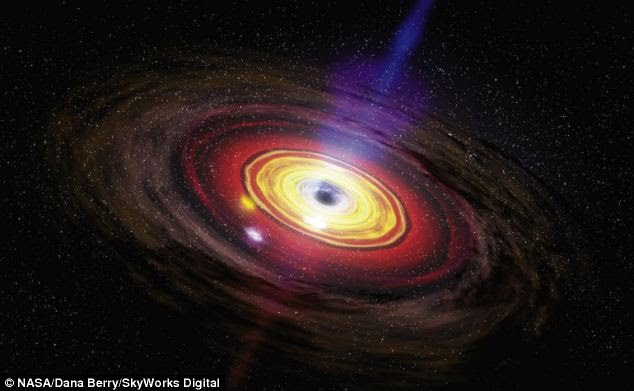
\includegraphics[height=30cm,width=21cm,angle=-45]{Figure/accretion_disk.jpg}}


\title{\vspace{15mm}\fontsize{30pt}{16pt}\selectfont\textbf{Master Thesis: \\Dust reverberation mapping of AGN in the local universe}\vspace{120mm}} % Article title

\author{
\fontsize{24pt}{16pt}
%\large
\textsc{Lynge R. B. Lauritsen} \\
\normalsize University of Copenhagen \\ % Your institution
\date{August 2018}
\vspace{-9mm}
}
%----------------------------------------------------------------------------------------


\usepackage{amsmath}
\begin{document}
\begin{titlepage}
%\begin{multicols}{1}
\color{white}
\maketitle % Insert title
\pagenumbering{gobble}
\clearpage
%\end{multicols}{}
\end{titlepage}

%\thispagestyle{fancy} % All pages have headers and footers

%----------------------------------------------------------------------------------------
%	ABSTRACT
%----------------------------------------------------------------------------------------

%\begin{abstract}

%\noindent ABSTRACT

%\end{abstract}

%----------------------------------------------------------------------------------------
%	ARTICLE CONTENTS
%----------------------------------------------------------------------------------------
%\begin{multicols}{2} % Two-column layout throughout the main article text
\color{black}
\newpage
\tableofcontents
\pagenumbering{gobble}
\clearpage
\newpage
\pagenumbering{arabic}


\section{Introduction}
This paper will discuss the use of Reverberation Mapping of AGN Light Curves on quasars observed using the Rapid Eye Mount (REM) telescope in the La Palma site in Chile. The aim of this paper is to demonstrate the possibilities in using observation from different bands to determine the driving function of the quasars' as well as all relevant transfer functions. It will discuss the process of determining the light curves based on local standard stars, as well as the creation and running of the MCMC algorithm used to determine the relevant constants of the transfer functions.\\
\\
The project has been approached as two part. Initially the aim was to produce reliable light curves from the observational images obtained by the INAF Rapid Eye Mount (REM) Telescope at the La Silla observatory site in Chile. The observations from REM are done across the J,H,K,g,r,i,z bands. The second part of the project consists of creating a python program capable of determining the UV-continuum light curve of the AGNs and the associated transfer functions, and thusly the lag-times. \\

\section[Relevance of AGN in cosmological measurements]{Relevance of AGN in cosmological measurements\footnote{Apart from the, when relevant, specified papers this section relies heavily on Mo, Bosch and White 2010, Carroll and Ostlie 2014 and Neal Jackson \emph{The Hubble Constant} 2015}}
Edwin Hubble showed a relationship in cosmological measurements between distance and redshift (\emph{equation \ref{eq:redshift}}), and thus concluded that the recession velocity of astronomical objects not bound gravitationally was a function of distance. This is explained by the theory of the expanding universe.
\begin{equation}
z = \frac{\lambda}{\lambda_{0}}-1
\label{eq:redshift}
\end{equation}
The motion of galaxies as they experience the expansion of the universe is called \emph{the Hubble flow}. Galactic movements can be described by two distinguishable motions. The locally influenced velocity \emph{through} space, called their \emph{peculiar velocity}, often associated with gravitational interactions with other galaxies, and the movements spawned and maintained through the expansion of the universe, the \emph{recessional velocity}. The latter is not due to galactic motion through surrounding space, rather it is the galaxy being "\emph{carried}" along with the surrounding space due to the expanding universe. Similarly the \emph{Cosmological redshift}, caused by the expanding universe, is not an expression of the observed galaxy movement by itself, but rather an expression of the light wave being "\emph{stretched}" as the universe expands along the path traveled by the wave. The knowledge of the expanding universe and the \emph{Hubble Constant} ($H_{0}$) allows the calculation of inter-galactic distances of non-gravitationally bound systems by calculating the redshift (\emph{equation \ref{eq:H_dist}}) and is called the \emph{Hubble law}.
\begin{equation}
d \simeq \frac{c}{H_{0}} \frac{(z+1)^{2}-1}{(z+1)^{2}+1}
\label{eq:H_dist}
\end{equation}
The main difficulty in utilising the Hubble Law is the determination of the Hubble Constant. This is historically a difficult calibration due to the importance on the accurate determination of the distance to remote galaxies, through secondary distance indicators, as well as the peculiar velocity of the observed galaxies. Additional uncertainty can occur due to the skewing of statistics originating from the \emph{Malmquist bias}, which is the bias inherent in Magnitude-limited samples, causing the astronomers to look only below a given apparent magnitude, thus as the distance increases only object of increasing absolute flux will be included. \\
\\
The increasing accuracy in the measurements of the Hubble constant from the local universe in the last half a decade has led to the realisation of a significant discrepancy between the measurements obtained from the observations of the local universe through measurements obtained from Cepheids and Type Ia Supernovae (SNe Ia) with $H_{0}=73.24 \pm 1.74\ km\ s^{-1}Mpc^{-1}$ (Riess et al. 2016), $H_{0}=72.8 \pm 2.4\ km\ s^{-1}Mpc^{-1}$ (Bonvin et al. 2017), $H_{0}=71.0 \pm 2.8\ km\ s^{-1}Mpc^{-1}$ (Arenas et al. 2017) and $H_{0}=73.48 \pm 1.66\ km\ s^{-1}Mpc^{-1}$ (Riess et al. 2018). In the opposite end of the observable universe, at the sound horizon Cosmic Microwave Background (CMB) observations, combined with a flat $\Lambda$CDM cosmology by the Planck Collaboration et al. (2016) determined the $H_{0}$ value to be $H_{0}=66.93 \pm 0.62\ km\ s^{-1}Mpc^{-1}$, and previous Planck releases has determined comparable values. This is a discrepancy of $3.4\sigma$ (Riess et al. 2018) and thus disagreement provides evidence of physics not included in the \emph{Standard Model}. The Standard Model does not include, among other theories, features such as \emph{Time-dependent or early dark energy}, \emph{Gravitational physics beyond general relativity}, \emph{additional relativistic particles} or \emph{non-zero curvature}, despite the main argument for their exclusion being the attempt at simplicity (Riess et al. 2016). It is beyond the scope of this project to investigate or explain the intricacies of the standard model, and the excluded physical theories, it is however of interest to the purpose of this project to understand the role AGN, or at further distances Quasars, can play in the future investigations into the Hubble Constant.

\subsection[Measuring the Hubble Constant in the local universe]{Measuring the Hubble Constant in the local universe\footnote{Apart from the, when relevant, specified papers this section relies heavily on Mo, Bosch and White 2010, Carroll and Ostlie 2014 and Neal Jackson \emph{The Hubble Constant} 2015}}
The Hubble Constant is as shown in \emph{equation \ref{eq:H_dist}} dependent upon the distance to the observed galaxy and the recession velocity of said galaxy. Thus calculation of the Hubble Constant necessitates an accurate determination of both these parameters. The recession velocity can typically be calculated through the redshift (\emph{equation \ref{eq:redshift}}), assuming the recession velocity dominates over the peculiar velocity. The relative error in the recession velocity, due to the peculiar velocity, is decreasing by distance as the recession velocity gains dominance. It is assumed that the relative error caused by the peculiar velocity decreases to under $10\%$ at distances in excess of $50\ Mpc$. The main difficulty in calculating an accurate value of the Hubble constant, based on observations of the local universe, originates in the issues inherent in distance measurements. The common method of distance estimation in the local universe, not utilising the Hubble law, is through the use of either \emph{standard candles} or \emph{standard rulers}. A \emph{standard candle} is an astronomical object of known, or accurately predictable luminosity, and a \emph{standard ruler} is an object of known or accurately predictable size. The determination of usable standard candles and/or rulers is a non-trivial issue, due to the significant spread in size and luminosity of galaxies and stars, regardless of their colour. Thus the perfect object for calculation of the Hubble constant is an object that
\begin{itemize}
\item has physical properties allowing the identification as a standard candle or ruler
\item can be independently calibrated e.g. does not build upon previous distance or luminosity determinations (a one-step process), as errors stack
\item at sufficient distance that error associated with peculiar velocity is small
\item astrophysically simple i.e. distance determination is independent on internal properties of the object
\item determines the Hubble constant independently of other cosmological parameters.
\end{itemize}
There are a number of \emph{one-step} methods of determining the Hubble constant. A full discussion of the various modes of Hubble determination in the local universe is somewhat outside the scope of this paper. Thus only the \emph{Megamaser cosmological method} will be discussed, due to its  familiarity with AGN cosmology, but neither the \emph{Sunyaev-Zel'dovich effect} nor the \emph{Gravitational lens model} will be discussed, however a full description is found in Neal Jackson \emph{The Hubble Constant} (2015). \\
\\
The \emph{Megamaser cosmological method} relies on the use of Very Long Baseline Interferometry (VLBI) of frequencies around $\nu \simeq 22\ GHz$, allowing resolution on the milliarcsecond scale. The Megamaser system in galaxies involves clumps of gas circulating the central galactic Supermassive Black Hole at radius $r \sim 0.1\ pc$. It becomes possible, in not too distant galaxies, to resolve the rotating clumps, and through continuous observation determine the clump velocities and accelerations. If one is to assume a Keplarian motion of the observed gas it becomes possible to determine the radius of the rotating gas, and the SMBH mass. This allows a trigonometric determination of the galactic distance, and thus a Hubble constant determination by comparing the galactic redshift with the distance obtained by the \emph{standard ruler}, that is the Megamaser system. This method however is vulnerable to systematic errors, although assumed to be small, originating from the understanding of the physical parameters of the disk, such as eccentricity, position angle, periapsis angle and inclination. \\
\\
The more traditional method of determining the distance to astronomical objects in the local universe is through the \emph{Local Distance ladder}. This approach relies on gradually expanding the distance estimation though understanding of the observed behavior of specific astronomical objects relative to comparable objects at already known distances, thus it becomes a ladder
\begin{enumerate}
\item {\bf \emph{Paralax approach:}} Close stars will change angle in the sky dependent on the Earth position in its orbit around the sun. The paralax approach thus relies on the observed motion of close stars on the sky, relative to more distant stellar objects. The \emph{parsec} ($pc$) is defined as the distance an arbitrary star must be from the solar system to achieve a $1\ arcsec$ angular change due to the Earth orbit. 
\item {\bf \emph{Open Clusters:}} The Paralax approach can be used to accurately determine the distance to close open clusters with an error $<1\%$. The stellar population of open clusters can be fitted on a \emph{Hertzsprung-Russell diagram} of the stellar temperature (determined through stellar colour and Wien's law) against apparent magnitude, revealing a characteristic sequence of stars, the so-called "main sequence stars". These nearby clusters can then be utilised in the calibration of distance to clusters outside the reach of the Paralax approach through "\emph{main sequence fitting}". This method can be applied to nearby galaxies, in which it is possible to resolve individual stars, such as the Large and Small Magellanic Clouds and is liable to have errors of a few percent.
\item {\bf \emph{Cepheids:}} The open cluster approach allows for the calibration of Cepheid variable stars. These stars is the intrinsically most luminous of the variable stars. Cepheids are pulsating Giant Blue stars located in a narrow range on the Hertzsprung-Russell diagram between $7000-8000\ K$. Observations show that the pulsation period is directly proportional with the luminosity, thus creating a standard candle, that can be calibrated through Cepheids observed in, or nearby to, open clusters. They are observed in the Large Magellanic Cloud and in galaxies at distances up to $20-30\ Mpc$, still significantly closer than the recommended $d>50\ Mpc$ for Hubble constant calibration.
\item {\bf \emph{Type Ia Supernovae (SNe Ia):}} A binary system of a Giant star dumping mass onto a white dwarf triggering a Supernovae explosion. The Type Ia SNe has same characteristic of the observed time-dependent light curve regardless of distance, and despite variation in the absolute luminosity between separate events, the similarities in light curves and the well understood degree of fading in the $15\ days$ following peak brightness ($m_{15}$) allows for the calibration of SNe Ia events for distance measurements, it they can be observed in galaxies with well calibrated Cepheid distances. Due to the brightness of the SNe Ia event this allows further distance calibration of galaxies, past the $d=50\ Mpc$ line at which the peculiar velocity driven error on the recession velocity decreases to $<10\%$.
\item {\bf \emph{Other relations:}} The SNe Ia is not the only distance measurement usable in the attempt to estimate distances in the local universe. The \emph{Tully-Fisher relation} allows for luminosity estimation of edge-on spiral galaxies through the relation $L \propto v^{4}$, similarly the elliptical galaxies has the \emph{Faber-Jackson relation}. There are several more complex methods of measuring distances to galaxies, however an in-depth discussion is not relevant.  
\end{enumerate}
The main issue arising from the Local Distance ladder is the stacking of uncertainties, thus any uncertainty at the early stages of the ladder will propagate through the ladder. 

\subsection[The Hubble constant and reverberation mapping]{The Hubble constant and reverberation mapping}
The main problematic of the Local Distance Ladder, with respect to determining the origin of the $3.4\sigma$ tension between the locally determined Hubble constant, and the CMB determined value, is the limited reach of the ladder, as well as the propagating uncertainties. Thus it becomes relevant to attempt to identify possible standard candles, or rulers, available in one-step jumps at larger distances. Despite the AGN or, at larger distances, Quasars being the most powerful observables in the known universe, their functionality as standard candles are non-existent due to the varying luminosity, while having a mostly unchanging SED thus not allowing for luminosity predictions to be made through the SED (Risaliti and Lusso 2015). AGNs are however excellent for high redshift observations, and thus if the internal dimensions of the AGN can be accurately determined, and then resolved, it would become possible to accurately utilise the observed AGN as a standard ruler, and thus allow determination of the Hubble constant at increasing redshift. \\
\\
This project aims at determining the inner scales of observed AGNs through the use of reverberation mapping. It is the aim of this project to lay the groundwork for an algorithm that can be utilised for \emph{reverberation mapping} of AGN without complete knowledge of the X-RAY driving function. If such an endeavor should prove successful it would allow for future $H_{0}$ calibrations to provide a deeper understanding of the expansion of the apparent tension in the local and CMB measurements by providing a means of determining the Hubble constant at longer redshifts. 



\section{Active Galactic Nuclei}
Active Galactic Nuclei, or AGN for short, is used to describe powerful energetic and luminous phenomena in the galactic center that does not originate from the galactic stellar population. It is generally believed that these phenomena is powered by accretion onto a Supermassive Black Hole (SMBH). This accretion however radiates in the X-RAY bands, rather than the optical and NIR bands studied in this project. Therefore it becomes of paramount importance to understand the workings of the AGN and the various processes by which light is emitted. This section will thus discuss the AGN phenomena, how it originates as well as its importance in modern astrophyics.

\subsection{Observing and identifying the AGN}
AGN identification and observation historically follow a list of observable properties. The earlier identification methods as used by both Schmidt (1969) as well as Peterson (1997) and later Peterson (2008) allows AGN identification based upon datasets of similar nature as the ones used in this project. These identification properties is; 
\begin{enumerate}
\item The pointlike representation of an AGN upon an imaging detector
\item Strong emission lines
\item The Continuum Luminosity varies over time
\item Evidence of strong non-stellar emission
\item Strong X-RAY emission
\item Radio emission
\item Non-stellar UV through IR emission
\item Broad emission lines in the UV through IR.
\end{enumerate}
it is important to note however that not all observables is always registered. In the datasets providing the foundation for this project the observed AGN appear as point-like, time-varying emission in the center of resolved galaxies (the so-called Seyfert Galaxies discussed later). 
\\
\subsection{AGN morphology}
It can generally be said that AGN falls into two different categories. The Seyfert Galaxies and the Quasars. These categories each have identifying points, however it is somewhat unclear to which degree they are distinctly different objects, or if the difference is mostly due to possibilities of observation. The distinction is of general importance and interest, however for the majority of this project it makes little actual difference in the results obtained, although it should be said that the available data did belong to Seyfert galaxies. 

\subsubsection{Seyfert Galaxies}
Discovered by Carl Seyfert (1943) these galaxies are Active Galaxies characterized by being spiral galaxies with a bright star-like nuclei in the center. Spectroscopically these galaxies contains both non-thermal continuum radiation and broad emission lines in their spectra. In addition observations show that the Luminosity output from the Nuclei originating in these Active Galaxies can at times vary by more than a factor of two in a year. \\
\\
The first Active Galaxy observed in 1908 by E. A. Fath at the Lick Observatory was NGC 1068. However not until 1943 did Carl Seyfert identify these as a distinct class of galaxies, now called Seyfert Galaxies. Not until the late 1950's did these galaxies become relevant again, with their identification as radio sources. Woltjer (1959) identified these Seyfert galaxies as having:
\begin{enumerate}
\item Unresolved nuclei, so at the then observational quality, a nucleus smaller than 100 pc. 
\item Lifetimes in excess of $10^8$ years. This being concluded from the realisation that Seyfert Galaxies makes up 1/100 of all spiral galaxies. Leading to two possible conclusions. Either all Spiral Galaxies pases through a Seyfert phase, or they are fundamentally different from other spirals, making it logical to assume they have lifetimes comparable to other spiral galaxies (of order $10^{10}$ yrs).
\item If it is assumed the material in the Nucleus is gravitationally bound, then based on the widths of the emission lines (excess of $10^3$ $kms^{-1}$) and the viral argument \emph{equation \ref{eq:Viral}},

\begin{equation}
M \approx \frac{v^2r} {G}
\label{eq:Viral}
\end{equation}
then it must be assumed the Mass of the Nucleus is of the order $10^6$ $M_O$.
\end{enumerate}
It is of note that the Seyfert Galaxies fit into two types. Seyfert I galaxies has permitted emission lines originating primarily from Hydrogen with very broad characteristics and giving FWHM corresponding to velocities in excess of $10^3$ $kms^{-1}$. Additionally the Seyfert I galaxies also contain forbidden lines (such as [OIII]) with much narrower profiles ($10^2-10^3$ $kms^{-1}$). Seyfert II galaxies differs in that the emission observed is originating in the Narrow Line Region (NLR) entirely. This does not necessarily imply an absence of a Broad Band Region (BLR), as this region could be unobservable in this galaxy. \\
\\
Most galaxies contains a Supermassive Black Hole (SMBH) in their center, however only few becomes Seyfert Galaxies. Studies seems to suggest that the SMBH becomes "active" due to disturbances in the gravitational potential, caused by either tidal interaction with foreign galaxies or galactic mergers. It is suggested that the disturbances in the gravitational potential is essential for the gas to overcome the angular momentum barrier (discussed later), allowing the accretion of gas onto the SMBH (Schneider 2006).

\subsubsection{Quasars}
Quasars, or as originally called Quasi-Stellar Radio Source, are the most luminous AGNs observed. A subset of these are also strong radio sources (5-10\%), and it was originally these objects that defined the quasars distinction and name. Generally quasars have strong similarities with Seyfert Galaxies, however they have very weak stellar absorption features and the Narrow Lines tends to be weaker when compared to the Broad Lines than observed in the Seyfert Galaxies. The optical spectrum observed from quasars are similar to those observed in the Seyfert Galaxies. In formal classification the distinction is made from the absolute magnitude with \emph{equation \ref{eq:quasar_distinction}} defining a quasar.
\begin{equation}
M_{B} \le -21.5 + 5log(h_{0}) 
\label{eq:quasar_distinction}
\end{equation}
This distinction is however a historical construct, based upon the observable qualities of the respective AGNs, as it appears the only fundamental difference between Quasars and Seyfert Galaxies is the Luminosity of the object. The quasar Luminosity can be of the order $10^3$ larger than that of a galaxy, and therefore only at low redshift high resolution quasars will the host galaxy be observable.[CHAPTER 14 GALAXY FORMATION AND EVOLUTION]

\subsubsection{Radio Galaxies}
The normal spiral galaxies will have weak radio emission (mostly powered through SN remnants) and therefore have power (\emph{equation \ref{eq:SN_radio}}),

\begin{equation}
P_{1.4GHz} \le 2*10^{23} WHz^{-1}
\label{eq:SN_radio}
\end{equation}
this allows the definition of radio galaxies of being galaxies with $P_{1.4GHz}$ larger than \emph{equation \ref{eq:SN_radio}}. \\
\\
Radio Galaxies were originally identified through the third survey at Cambridge, and it has since been realised that almost all radio galaxies are AGN ellipticals. Much like the Seyfert Galaxies two types are identified, the Broad-Line Radio Galaxies (BLRG) and Narrow-Line Radio Galaxies (NLRG). The BLRG and NLRG differs from their corresponding Seyfert Galaxies partly in being radio loud, and the morphology of the host galaxy, but also in the existence of mostly asymmetric stretching radio jets stretching several hundred kiloparsec or even megaparsec from the AGN. \\

\subsection[Stellar radiation]{Stellar Radiation\footnote{This section is build upon Léna, Rouan, Lebrun \& Pelat 2012 and Schneider 2006}}
An understanding of the observed properties of stars becomes necessary to identify, and understand the properties of AGNs. The most important characteristic of the AGN spectrum utilised in this project is the \emph{non-stellar} characteristics of the radiation emitted by the AGN. The \emph{AGN Radiation Spectrum} differs from the \emph{Stellar Radiation Spectrum} by both the varying luminosity created by the AGN, as opposed to the constant Luminosity Function from the Stellar Light-Source, and the non-\emph{Black Body Radiation} of the AGN. \\
\\
Despite the lack of any astronomical objects emitting like a perfect \emph{Black Body}, observations show that it is a good first order approximation for the spectral energy distribution of \emph{stellar radiation}. Thus the specific intensity ($B_{\nu}$) of the stellar radiation can be approximated by the \emph{Planck law} %(see \emph{equation \ref{eq:planck}}).
\begin{equation}
B_{\nu}(T) = \frac{2h\nu^{3}}{c^{2}}\bigg[e^{\frac{h\nu}{kT}}-1\bigg]^{-1}.
\label{eq:planck}
\end{equation}
In the model of the radiation emitted by a star is described as a Black Body spectrum the luminosity ($L$) is dependent on the temperature ($T$) and radius ($r$) of the star
\begin{equation}
L = 4\pi r^{2}\sigma_{SB}T^{4},
\label{eq:star_L}
\end{equation}
with $\sigma_{SB}$ being the \emph{Steffan Boltzmann constant}. Thus the \emph{effective temperature} ($T_{eff}$) is often discussed, as the temperature of a Black Body, of identical radius, emitting the same luminosity and spectral energy distribution as the star. \\
\\
Additionally stellar observations identify the relationship between stellar luminosity and stellar mass as being
\begin{equation}
\frac{L}{L_{O}} = \bigg(\frac{M}{M_{O}}\bigg)^{3.5},
\label{eq:star_L_M}
\end{equation}
and thus a main-sequence star of mass $10M_{O}$ emits $\sim3200L_{O}$. This increase in luminosity causes a decrease in the main-sequence lifetime following
\begin{equation}
t_{MS} = 8\times 10^{9}\bigg(\frac{M}{M_{O}}\bigg)^{-2.5} yr.
\label{eq:star_ms_life}
\end{equation}
Thus the previously mentioned star would have a main-sequence lifetime of $t_{MS}\sim 2.5\times 10^{7}\ yr$. 


\subsection{AGN structure}
The AGN is the most powerful and luminous objects known in the universe. Evidence shows quasars as early as redshift $z=7$, leading to a formation time-scale of the first AGNs of $t_{AGN}<0.5\ Gyr$ (Mo, Bosch and White 2010).The AGN, being the most powerful astronomical process known, is the cause of a massive energy output throughout its lifetime. Some of the most powerful AGNs known has an energy output, integrated over their entire lifetime, of $E\geq 3\times 10^{61}\ erg$. Such massive energy outputs can only be generated through nuclear processes or accretion of matter. It is however not feasible for the energy output to be the result of nuclear fusion, as in the stellar core, as this has an efficiency of around 0.007 (Mo, Bosch and white 2010). This efficiency ($\epsilon$) for converting mass to energy, when applied to Einsteins equation means $E=\epsilon mc^{2}$ necessitating the mass of a Black Hole fueled by fusion of $2\times 10^{9}\ M_{O}$ (Schneider 2006). This far exceeds the upper limit of $150\ M_{O}$ observationally determined for the stellar mass for our local universe (Weidner \& Kroupa 2004), as well as following \emph{equation \ref{eq:star_ms_life}} it becomes apparent that the expected stellar lifetime would be far too short, making it unfeasible for the AGN to be powered by nuclear fusion. In comparison, however, the accretion process of free-falling material onto a Black Hole devoid of angular momentum has an efficiency of around 0.06 and in the case of the accreting material onto a Black Hole being subject to the maximum rotation allowed the accretion can be as large as 0.29 (Schneider 2006). Thus it is most feasible of the AGN to be powered through the accreting method, both due to the higher efficiency and the high mass of the AGN being far higher than any observed, or theorised, stars. This leads to the theory of accretion onto a SMBH with the AGN situated around a SMBH being the accepted theory. In this accretion theory the AGN is powered by gas being accreted onto the central SMBH. The energy originates from the potential energy stored in the accretion disk with respect to the SMBH. 

\subsubsection{The Driving Engine}
It is assumed that the energy output from an AGN is generated by accretion onto a Supermassive Black Hole (SMBH), this is generally called the \emph{Supermassive Black Hole Paradigm}. In this model the energy source from the AGN is the potential energy release as material is accreted from the accretion disk onto the SMBH. \\
\\
\paragraph[The Black Hole:]{The Black Hole:\footnote{This section build heavily on Mo, Bosch and White 2010}}\mbox{}\\
In the case of gaseous material surrounding an energy source like a star or AGN, in a spherical geometry, the surrounding material will experience an outward pressure scaling with the luminosity ($L$) and inversely proportional with the radius ($r$) squared,
\begin{equation}
P_{rad}(r) = \frac{L} {2\pi r^{2}c}
\label{eq:P_rad}
\end{equation}
thus in a region of ionized gas, like the one created by the photo-ionization from stars and AGN, the pressure will exert a force on the gas due to the scattering of photons by electrons given by,
\begin{equation}
\mathbf{F_{rad}} = \sigma_{T}P_{rad}(r)n_{e}(r) \mathbf{\hat{r}} = \frac{\sigma_{T}Ln_{e}(r)}{2\pi r^{2}c}\mathbf{\hat{r}}
\label{eq:F_rad}
\end{equation}
with $\sigma_{T}$ being the Thomson scattering cross-section ($\sigma_{T} = \frac{8\pi}{3}r_{0}^{2}$) and $n_{e}(r)$ the electron density at radius $r$. Thus, if the cloud surrounding the AGN has to be maintained, it must be assumed that it is held by the gravitational potential of the AGN and thusit must be true that
\begin{equation}
|\mathbf{F_{rad}}| \le F_{grav} = \frac{GM_{BH}\rho(r)} {r^{2}},
\label{eq:F_grav}
\end{equation}
with $G$ being the gravitational constant, $M_{BH}$ the mass of the Black Hole and $\rho(r)$ the density of the gas. Thus the maximal accretion luminosity that can be reached by this spherical accretion, the Eddington Luminosity ($L_{Edd}$), can be found to be
\begin{equation}
L_{Edd} \equiv \frac{4\pi Gcm_{p}}{\sigma_{T}}M_{BH},
\label{eq:L_Edd}
\end{equation}
with $m_{p}$ being the proton mass. A SMBH does not necessarily accrete at the Eddington Luminosity, thus assuming an \emph{accretion rate} of $\dot{M}_{BH}$, where the meterial being accreted crosses a shell at radius r, the AGN luminosity can be calculated as
\begin{equation}
L_{AGN} = \frac{GM_{BH}} {r}\dot{M}_{BH}.
\label{eq:L_AGN}
\end{equation}
The Schwarzshild radius, or gravitational radius, of Black Holes ($r_S$) is given as
\begin{equation}
r_{S} = \frac{2GM_{BH}} {c^{2}},
\label{eq:r_S}
\end{equation}
and is the radius at which the escape velocity in the solution to the viral theorem exceeds the speed of light ($c$). The Schwarzshild radius can be used to determine the efficiency at which accretion occurs, or given the latter the radius at which it occurs
\begin{equation}
\epsilon_{r} = \frac{L} {\dot{M}_{BH}c^{2}} = \frac{1}{2}\frac{r_{S}}{r}.
\label{eq:epsilon_r}
\end{equation}
Observations indicates that the continuum radiation from AGNs originates primarily from $r\sim5r_{S}$. Thus the efficiency at which mass is converted into radiation is around 0.1. Thus it must be concluded that the Black Hole is rotating to induce a higher mass conversion efficiency than the non-rotating Black Hole efficiency of 0.06.  \\
\\
\emph{The Accretion Disk:}\footnote{This section build heavily on Schneider 2006} \\
Accretion is the process at which material fall onto a compact object, such as a protostar or a Black Hole. During this process the gravitational potential energy of the material is converted into kinetic energy. In the case of unimpeded accretion there will be no release of radiation, as AGNs are some of the most energetically powerful and luminous objects in the universe the accretion cannot be unimpeded. This impediment is provided through the laws governing conservation of angular momentum ($L=I\omega$), as the gas, and other material, orbiting in galaxies, also in the galactic center, has a finite angular momentum, and, as angular momentum is always preserved, free-fall accretion onto the Black Hole is prohibited. Gas particle friction, from the viscosity of the materials, resulting in angular momentum transfer will result in a disk like structure, perpendicular to the direction of the angular momentum. It is possible to view the disk as a series of concentric rings all rotating with approximately the Kepler velocity (\emph{equation \ref{eq:Kepler_velocity}})
\begin{equation}
v_{Kepler} = \sqrt{\frac{GM_{BH}}{r}}
\label{eq:Kepler_velocity}
\end{equation}
causing friction between them, causing heating of the disk. This heating de-accelerates the gas causing inward motion of the material. This inward motion provides released potential energy, which in turn is the energy observed being radiated away as thermal radiation. \\
\\
Thus when the mass m in the accretion disk moves from radius $r+\Delta r$ to radius $r$, the energy generated will be
\begin{equation}
\Delta E_{pot} = \frac{GM_{BH}m}{r+\Delta r} - \frac{GM_{BH}m}{r} \approx -\frac{GM_{BH}m\Delta r}{r^{2}}.
\label{eq:pot_E_loss}
\end{equation}
\emph{Equation \ref{eq:pot_E_loss}} assumes that the SMBH mass is dominant in the system, as to ignore the self-gravitational potential energy of the accretion disk itself. The viral theorem dictates that half the converted energy generates kinetic energy, and the second half can be lost in internal energy. If the energy released is emitted locally in the disk the luminosity release of the disk as a result of mass m moving a radial distance of $\Delta r$ is
\begin{equation}
\Delta L = \frac{GM_{BH}\dot{M}_{BH}}{2r^{2}}\Delta r.
\label{eq:delta_L}
\end{equation}
$\dot{M}_{BH}$ is radially independent as to avoid accumulation of material at any given radius, and thus all concentric rings of width $\Delta r$ experiences a mass flow of $\dot{M}_{BH}$. In the case of optically thick disks the radiation emitted will become Black Body radiation, thus \emph{equation \ref{eq:delta_L}} becomes
\begin{equation}
\Delta L = 2\times 2\pi r\Delta r\sigma_{SB}T^{4}(r),
\label{eq:delta_L_BB}
\end{equation}
with $\sigma_{SB}$ denoting the Steffan-Boltzman constant and the factor 2 the double sided nature of a disk. Thus determining the actual temperature of the disk becomes relevant in order to accurately calculate the emitted luminosity. This question is two sided. In the case of $r_{S}<<r$
\begin{equation}
T(r) = (\frac{3GM_{BH}\dot{M}_{BH}}{8\pi\sigma_{SB}r^{3}})^{1/4},
\label{eq:T_r_s_less_r}
\end{equation}
and in the case of the former condition not being true the temperature is given by
\begin{equation}
T(r) = (\frac{3c^{6}\dot{M}_{BH}}{64\pi\sigma_{SB}G^{2}})^{1/4}M_{BH}^{-1/2}(\frac{r}{r_{S}})^{-3/4}.
\label{eq:T_r}
\end{equation}
The disk emission is, due to the temperature increasing $\propto r^{-3/4}$, to a first order approximation a superimposition of concentric black body rings at differing temperatures. Additionally the temperature increases at increased accretion rate, and lowers at more massive black holes. This explains the lack of X-Ray emitted from AGN accretion disks due to thermal radiation, as opposed to X-Ray binaries such as neutron stars and stellar-mass black holes. 	

\subsubsection[Broad-Line Region]{Broad-Line Region\footnote{Unless otherwise referenced this section build heavily upon Bianchi, Maiolino \& Risaliti \emph{AGN Obscuration and the Unified Model} 2012, Schneider 2006, Peterson 1997 and Mo, Bosch and White 2010.}} \label{BLR}

The Broad-Line Region (BLR) is located in a halo surrounding the accretion disk, and is observable in the optical spectra of Seyfert I galaxies, and in some Quasars, with strong emission lines with velocity width ($\Delta v$) of $500$ $kms^{-1} \le \Delta v\le 10\ 000\ km/s$. The observed velocity dispersion of the BLR emission lines could have two origins. Either the velocity dispersion originates through thermal velocity
\begin{equation}
v(T_{gas}) \approx (\frac{kT_{gas}} {m_{p}})^{1/2},
\label{eq:v_gas_T}
\end{equation} 
or the origin of the observed broadening of emission lines is attributed to the rotational motion of the gas in the BLR
\begin{equation}
v_{rot} \approx \sqrt{\frac{GM_{BH}} {r}} = \frac{c}{\sqrt{2}}\sqrt{\frac{r_{S}}{r}},
\label{eq:v_gas_T}
\end{equation}
thus becoming Doppler Broadening. In order to obtain such velocity dispersion from the temperature of the gas in the BLR, a gas temperature of the order $10^{10}$ $K$ would become necessary. This is not the case, as at this temperature all atoms would be fully ionized, eliminating all emission lines, as well as the lack of the elimination of the 511 KeV line in Gamma radiation, which would result from the plasma generated e$^{+}$e$^{-}$-pairs at such temperatures (Schneider 2006). Thus the velocity dispersion is Doppler Broadening of the emission lines, as a result of the rotational motion of the gas in the BLR, and thus a different method of estimating the gas temperature must be considered. The observed Doppler Broadening would be attainable a radii of $r \sim 1000r_{S}$ (Schneider 2006). \\
\\
%Thus the broadening of the emission lines must be attributed to Doppler Broadening, and thus it must be concluded that the gas in the BLR is rotating with velocities in the region $500\ km/s < v_{gas} < 10\ 000\ km/s$. The velocities present in the BLR is only attainable in the presence of a strong gravitational field and thus,
\noindent Despite the difficulty in determining the gas temperature originating in the BLR, due to electron densities being sufficiently large as to collisionally suppress almost all forbidden line emissions, the relative line intensities of ionized gases indicates a temperature of order $10^4$ $K$, corresponding to a velocity dispersion of $\approx$ $10$ $kms^{-1}$, leading further credence to the theory that the velocity dispersion is due to the Doppler Broadening. \\
\\%The profiles of the various emission lines can often in a low order approximation be described as a logarithmic evolution as a function of distance from the center of the AGN emission line (\emph{equation \ref{eq:log_emission_line}}).
%\begin{equation}
%F_{\lambda}(\Delta v) \propto -ln(\Delta v)
%\label{eq:log_emission_line}
%\end{equation}
%It is however not the case in all cases and different emission lines can vary significantly even in the same spectrum, and it is therefore an indication of the existence of 
The large Doppler broadening of the line observed in the BLR causes many of the normally observable features of a spectrum to become blended, and some features can become unresolved in the obtained AGN spectra. It is important to note that the emission lines varies with time dependent of the comparable variations in the continuum flux indicating a photoionization in the BLR driven by the central source (the SMBH). \\
\\
The gas density of the BLR can be estimated through the observed emission lines. While the forbidden transitions are all collisionally suppressed in the BLR, allowed and semi-forbidden lines are not. The distinction between allowed, forbidden and semi-forbidden emission lines are done by basis of quantum mechanical transitional probability, and thus the distinction can be used to predict the probability of de-excitation being through spontaneous emission rather than through collisional energy loss. Allowed transitions has high transitional probabilities, and thus short lifetimes (of order $t \lesssim 10^{-8}s$), thus reducing the chance of collisional suppression. Forbidden transitions by comparison have lifetimes typically around $1s$, with the semi-forbidden ones being somewhere between the two. Examples of allowed transitions observed in the BLR spectrum are $Ly\alpha$, $Mg_{II}$ and $C_{IV}$, with semi-forbidden ones being $C_{III}]$ and $N_{IV}]$. The \emph{mean free path ($\lambda$)} and thus the \emph{mean travel time ($\tau_{t}$)} of an ideal gas can be described through the gas radius ($d$), Avogadro's number ($N_{A}$), the temperature ($T$), the gas constant ($R$) and the gas pressure ($P$) and is given by\footnote{http://hyperphysics.phy-astr.gsu.edu/hbase/Kinetic/menfre.html}
\begin{equation}
\lambda = \frac{RT}{\sqrt(2)\pi d^{2}N_{A}P}.
\label{eq:mean_free_path}
\end{equation} 
Thus it can be concluded that the chance for collisional de-excitation is dependent on the physical conditions in the gas, while radiational transitions are dependent on the atomic parameters, and thus a well known quantity. Thus the lack of forbidden emission lines are indicative of the lower bound on the gas density, such as the [$O_{III}$] $\lambda 4363$, $\lambda 4959$ and $\lambda 5007$ transitions that is usually strong in ionized gases, but is suppressed at electron densities exceeding ~$10^{8} cm^{-3}$. Additionally the presence of the semi-forbidden lines can be utilised for estimation of the upper bounds for the gas densities. In Schneider 2006 the estimate of the electron density in the BLR gas is estimated at $n_{e} \sim 3\times 10^{9}\ cm^{-3}$ based upon $[O_{III}]$ and $C_{III}]$ lines. Further, the total number of emitted line photons can be measured using the AGN distance and the observed line strength. These calculations allows for determination of the total emitting volume from the BLR, and thus the BLR gas filling factor of $10^{-7}$. This indicated the BLR gas is concentrated in clouds of gas (Schneider 2006).  \\
\\
Observations comparing the continuum radiation of the central engine, and the BLR line emission flux indicates a fraction of $0.1$ of the AGN energy is being absorbed by the BLR. Thus it must be concluded that the total surface area of the BLR clouds, as they are optically thick, spans $10\%$ of the solid angle of the AGN. From this, combined with the filling factor it is found that there are of order $10^{10}$ clouds in the AGN with a typical size of $\sim10^{11} cm$ (Schneider 2006). \\
\\
This project occupies itself with the reverberation mapping of the AGN, although not the BLR itself. Reverberation mapping of the BLR occupies itself with determining the structure of the BLR by observing the BLR response to continuum variations. As the AGN driving function varies it must be assumed that the physical conditions in the BLR exhibits comparable variations. The reverberation mapping attempts to determine the transfer functions governing the delay between the UV-driving function variations of the AGN and the BLR response, which is governed by the light travel-time effects within the BLR ($\tau=r/c$). The strength of the reverberation mapping technique is its ability to work independently of assumed BLR geometry and infer the geometry through the BLR response to continuum variations. The reverberation mapping techniques is based upon a series of assumptions as described by Peterson (1993).
\begin{enumerate}
\item The Continuum emission originates at a single compact and central source. Thus follows the SMBH model of the AGN. 
\item The BLR has a small filling factor (the majority of the volume attributed to the BLR is a vacuum), hence photons are able to propagate freely inside the BLR. This seems to be supported by the low \emph{filling factor} of the BLR, and no evidence of is observed for an Inter-Cloud Medium scattering the wave fronts.
\item There is a simple relationship between the ionizing continuum and the observable UV/optical continuum flux.
\item The light travel-time $\tau_{LT}=r/c$ across the BLR is the most important time scale. 
\begin{enumerate}
\item The BLR variations as response to the continuum variations is short compared to $\tau_{LT}$
\item Significant geometrical changes to the BLR (dynamical time scale) happens over significantly larger time scales than the $\tau_{LT}$, $\tau_{dyn}$ can be estimated as the time taken for cloud of gas to cross the BLR; $\tau_{dyn} = r/\Delta v_{FWHM}$
\item $\tau_{rec}$, the time scale for the cloud to reprocess ionizing radiation, is virtually instantaneous
\end{enumerate}
\end{enumerate}
The observed light from the BLR at any given time (t) is the sum of the light emitted from all the isodelay surfaces in the BLR, with all parts of the sum being each surface reaction to the continuum level at different points in the past. If the BLR is assumed to be a thin spherical shell of radius $r$, with $\theta$ being the angle between the line-of-sight to the central source and and a vector to a given point on the BLR shell, then this given iso-delay surface has a intersection ring of radius $rsin\theta$ and area $2\pi r^{2}sin\theta d\theta$ (\emph{figure \ref{fig:BLR_iso_delay}}).
\begin{figure}[t!]
\centering
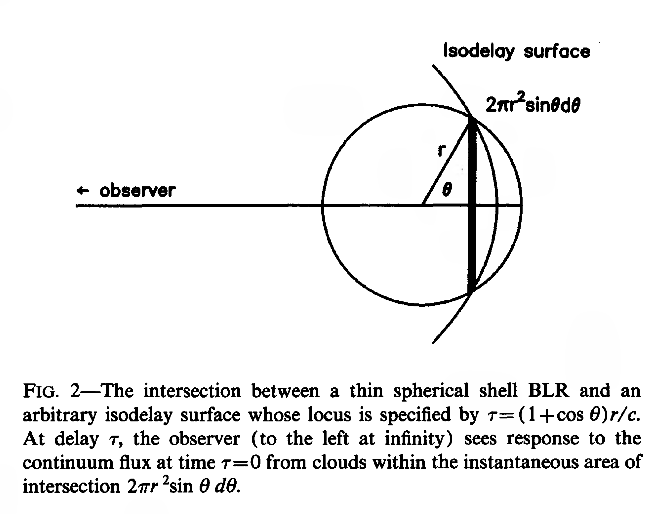
\includegraphics[width=1.00\linewidth]{Figure/BLR_iso_delay.png}
\caption{Figure from Peterson 1993.}
\label{fig:BLR_iso_delay}
\end{figure}
If we assume that the \emph{responsivity} ($\epsilon$) of all clouds are constant, the response to driving function variations can be written as a function of $\theta$ by 
\begin{equation}
\Psi(\theta)d\theta = 2\pi\epsilon r^{2}sin\theta d\theta.
\label{eq:theta_response_function}
\end{equation}
Thus any clouds on this iso-delay surface is observed with delay
\begin{equation}
\tau = (1 + cos\theta)r/c,
\label{eq:cloud_delay}
\end{equation}
thus following
\begin{equation}
d\tau = -r/c\times sin\theta d\theta.
\label{eq:d_tau}
\end{equation}
This allows the line response and thus the transfer function ($\Psi(\tau)$) to be determined as
\begin{equation}
\Psi(\tau)d\tau = \Psi(\theta)\bigg|\frac{d\theta}{d\tau}\bigg| = 2\pi\epsilon rcd\tau.
\label{eq:d_tau}
\end{equation}
In the case of the thin BLR shell described the transfer function will be constant and non-zero between $\tau = 0$ at $\theta = 180^{\circ}$ and $\tau=2r/c$ at $\theta = 0^{\circ}$ (Peterson 1993 and Peterson 1997). The actuality is that the BLR is vastly more complicated. It is probably better represented by continuous concentric circles of iso-delay surfaces, none of which are covered along the entirety of the shell due to the low \emph{filling factor}. \\
\\
The BLR, as previously discussed, owes its ionization and heating variations to the varying central continuum source of the AGN. As the central source luminosity varies in the AGN, so should the BLR emission line fluxes and physical conditions. The physical size of the BLR is finite and as such the BLR response to changes in the X-RAY-continuum will be delayed. This delay is examined using \emph{Reverberation mapping}. The delay $\Delta t$ of the BLR response correspond to the \emph{light travel time} across the BLR ($r/c$). Thus it becomes possible to measure the physical extend of the BLR based upon the delay in the response function,allowing the analysis of the individual \emph{iso-delay surfaces} of the BLR. Additionally in spectroscopic analysis it becomes possible to identify the delay caused in different line transitions and thus the possibility of analysing different parts of the BLR, given sufficient resolution (Schneider 2006).\\
\\
The BLR appears to scale with the luminosity of the AGN, much like would be expected in the assumption that the outer edge of the BLR and inner edge of the durst torus is defined by the sublimation radius, and thus depending on the energy output by the AGN. Additionally reverberation mapping indicates a varying ionization structure of the BLR as a function of the distance from the central AGN. Thus it appears the higher the ionization energy required by a transition, the smaller the radius, thus construing the BLR as an inhomogeneous region of the AGN. This is exemplified by the NGC5548 AGN (not investigated by this project) with a delay of $\Delta t\sim 12\ d$ for the $Ly \alpha$-transition and $26\ d$ and $50\ d$ for $C_{III}]$ and $Mg_{II}$ respectively. This is found through both the use of reverberation mapping, and cooperated by the Doppler broadening of the various lines, with high energy lines being broader. Thus it must be concluded through existing reverberation mapping investigations of observed AGNs that an inhomogeneous BLR is present, spanning a large radius ($r$) comprised of different "layers", as demonstrated by the radial dependence of ionizing transitions in the BLR (Schneider 2006). \\
\\


\subsubsection[Reverberation Mapping]{Reverberation Mapping\footnote{Schneider 2006 is used for additional information.}}
The sub-parsec scale structure of AGNs, driving engine, accretion disk and BLR, are unresolved even in the closest AGNs and as such reverberation mapping becomes a vital, and time consuming, tool in AGN investigations (Fausnaugh et al. 2017). It is the only tool available  that allows the study of the central engine of the AGN, irrespective of the telescopic spatial resolution. It utilises spectroscopic, and photometric, observations to determine the light travel time between different components of the AGN (Nuñez, Chelouche \& Kaspi 2018). Previously BLR reverberation mapping, for a highly simplified BLR model, was discussed, however the usefulness of this method spans further than the BLR. In this project the reverberation mapping will focus on the dust torus as well as the accretion disk. \\
\\
Reverberation mapping can be used, as already discussed, to determine the time delay between the hot continuum radiation of the accretion disk, and the broad-emission lines of the BLR or the dust torus. It is however an additional possibility to utilise this approach to map the accretion disk itself. The time delays in the different observed bands of the accretion disk can be used to determine the light-travel time ($\tau_{AD}$) across the adccretion disk, thus providing information regarding the size, and temperature of the disk (Nuñez, Chelouche \& Kaspi 2018). \\
\\
As the standard geometrically thin, optically thick, accretion disk theory has a $T \propto r^{-3/4}$ temperature, radius relation, it follows that the Black Body emission is highly spatially dependent. The inner, hot, parts of the accretion disk radiate UV emission in the range $\sim 10-3,000$ \emph{Å}, whereas the outer parts are emitting in the optical and IR spectrum of $\sim 3,000-10,000$ \emph{Å}. As the X-RAY emission from the corona, irradiating the disk, undergoes variations, the disk radiation must respond to the changed physical conditions. It must then be expected that a time delay, corresponding to the disk size, can be observed between the UV- and IR-emission (Fausnaugh et al. 2017 and Krolik et al. 1991). 
\begin{figure}[t!]
\centering
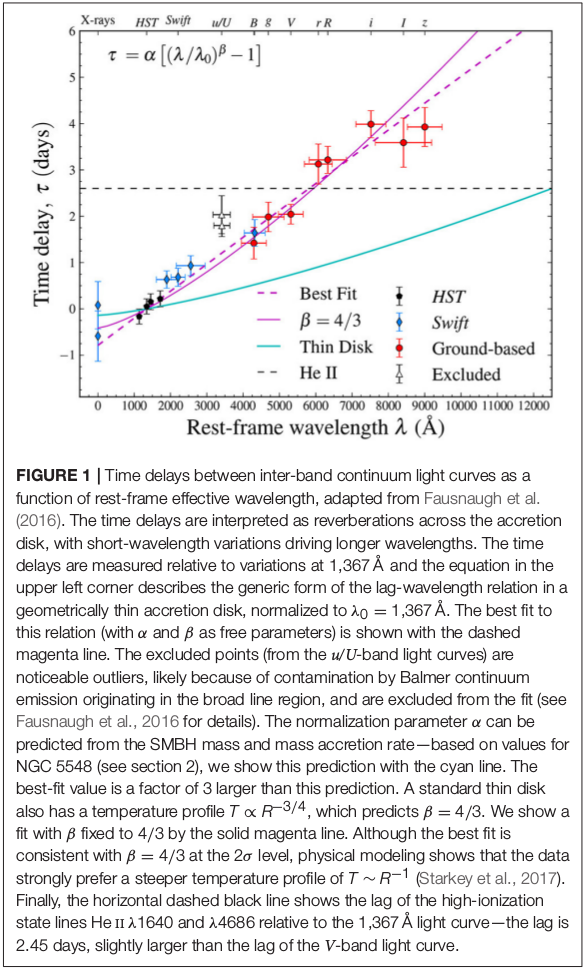
\includegraphics[width=0.5\linewidth]{Figure/Fausnaugh_AD_RM.png}
\caption{Image from Fausnaugh et al. 2017}
\label{fig:ad_rm_faugh}
\end{figure}
\\
\\
The results from Fausnaugh et al. 2017 (\emph{figure \ref{fig:ad_rm_faugh}}) indicates that the that the $T \propto r^{-3/4}$ may not be entirely accurate, and these results suggests a temperature profile of $T \propto r^{-1}$ may indeed be more accurate. This shows the importance of the reverberation mapping technique, in the ability to infer the disk structure without the capability to resolve the disk itself. The difficulty in reverberation mapping is the time scale of AGN variations. The variations occurring in the AGN luminosity happens over periods spanning from months to years, and as such any level of Reverberation mapping investigation must be based upon data collected over a period of years. \\
\\
In this project the reverberation mapping is utilised in an additional attempt to estimate and model the X-RAY driving function. This is done in an attempt to compensate for significantly more sparse sampling than that traditionally used. 
%Additionally to utilise the reverberation mapping technique to its fullest it becomes necessary to accurately monitor the continuum light curve, as generated through accretion onto the SMBH in the X-RAY spectrum. It is in part this problem this project simplify. This project aims to replicate the \emph{transfer functions} and the continuum emission of AGN based upon observation on various observational bands and thus allowing for cheaper and easier reverberation mapping. 




\subsubsection{Narrow-Line Region}
The Narrow-Line Region (NLR) are the largest spacial scale at which the ionizing radiation from the central engine is dominant. This region in the Seyfert Galaxies extends from $\sim 10 pc$ up to $\sim 1 kpc$, and thus exists on sufficiently extended spatial scales as to allow the physical and kinematic distribution to be mapped out to some extend. The NLR spectrum as opposed to the BLR spectrum contains emission lines from forbidden interactions, leading to the conclusion that the electron density is significantly lower, this also allows for the forbidden line emission from the NLR to be isotropic, due to the low chance of self-absorption of forbidden emission lines. Thusly it is possible by comparing the intensities of forbidden lines to determine physical properties of the NLR such as the temperatures and electron densities. An additional key difference between the BLR and NLR is the precense of dust in the latter, thus one can infer that the NLR is located outside the dust sublimation radius.\\
\\
The NLR shows as a bi-conical shape, owing to the presence of the dusty torus, at radii of $\sim 0.1 pc$ up to $\sim 10 pc$ from the central engine, which collimates the AGN radiation. Additionally due to the larger distance from the AGN center the emission line broadening of the NLR is significantly shorter, than the BLR, with $\Delta v_{FWHM} < 1000 kms^{-1}$.\\
\\
The physical conditions in the NLR can be inferred from the observed emission lines. Two key observable that it is possible to constrain well in the NLR as opposed to the BLR is the electron density and the electron temperature. In both cases emission lines originating from forbidden transitions from the same ion, to prevent bias in the result originating from the chemical composition of the NLR, is compared.

\begin{enumerate}
\item The electron densities are constrained using the forbidden transitions generating the $[OII] \lambda\lambda 3726,3729$ and the $[SII] \lambda\lambda 6716,6731$ emission lines. The $[OII]$ emission lines are rarely used in this respect however, due to the high degree of overlapping due to Doppler broadening. The electron density is given by \emph{equation \ref{eq:NLR_electron_density}},
\begin{equation}
j_{21} = n_{2}A_{21}\frac{hv_{21}} {4\pi}
\label{eq:NLR_electron_density}
\end{equation}\\
with $n_{2}$ being the number density af atoms at the n=2 state, $A_{21}$ the Einstein coefficient, $j_{21}$ is the emissivity in the line and $hv_{21}$ the transition photon energy.
\item The NLR electron temperature is determined by comparing emission lines from forbidden transitions from same ions at different exitation potentials ($\chi$), leading to the relative intensities being highly temperature dependent. Often used emission lines are $[OIII]\lambda\lambda 4363,4959,5007$ and $[NII] \lambda\lambda 5755,6548,6583$ although the $[NII] \lambda 5755$ relatively weak and therefore sub-optimal. The temperature is determined using \emph{equation \ref{eq:NLR_electron_T}}.
\begin{equation}
\frac{F(\lambda4959 + \lambda5007)} {F(\lambda4363)} = \frac{7.33e^{3.29\times10^{4}/T_{e}}} {1 + 4.4\times10^{-4}n_{e}T_{e}^{-1/2}}
\label{eq:NLR_electron_T}
\end{equation}
\end{enumerate}
Utilising the emission lines originating from forbidden transitions in the NLR typical values for the electron density and temperature is found to be; $10^{2} cm^{-3} < n_{e} < 10^{4} cm^{-3}$ with the average value around 2000$cm^{-3}$ and the temperature is found to be between 10,000 and 25,000 K and typically around 16,000 K. 


\subsubsection{Unification Theory}
The unification theory aims at providing a singular explanation for the AGN phenomena by attributing the observed differences to the conditions of the observation as opposed to intrinsic differences between the observed AGN phenomena. The possibility of the unification theory is based on the symmetric properties intrinsic in AGNs. The AGN symmetry is much like galaxies and solar systems not spherical, but rather AGN's are axisymmetric systems. This allows for differences in the observational result based upon the inclination angle of the system being observed. The Unification Theory gains credence due to the many similarities between Type I and Type II Seyfert Galaxies.  \\
\\
The Unification Theory assumes the AGN being powered by a central SMBH of order $10^6-10^{10} M_O$ that is surrounded by an accretion disk. Surrounding the accretion disk is  a region of hot, fast-moving dense gas, the so called BLR discussed earlier. In Type I Seyfert Galaxies this BLR is the cause of a significant amount of the observed Luminosity. In the Unification World view the BLR is photoionized by UV radiation from the central engine, the SMBH accreting from the accretion disk, and thusly the BLR emission lines changes intesity following changes in the UV continuum. \\
Surrounding the BLR is a dusty region with the inner radius being the sublimation radius from the SMBH. This is also the region called the Torus. This dusty region reprocesses the UV continuum emission and emits the energy in the IR regime. Further out is the Narrow line region comprised of cool and low density gas. In this region the velocity caused by the gravitational rotational motion is of the order $10^2 kms^{-1}$ and is located at pc scale distances from the central engine of the AGN.\\
\\
Thus it is possible under the Unification Theorem to represent Seyfert I and Seyfert II galaxies as being fundamentally identical, with the main difference being the inclination angle of the host galaxies, and thus in Seyfert II Galaxies the BLR is only not observed due to the energy being blocked by the orientation of the Torus. Additionally it would then stand to reason that Quasars are either Seyfert Galaxies with sufficiently bright AGNs as to overshadow the host galaxy, or sufficiently distant as to have the Luminosity from the host galaxy being undetectable or a combination of the two. \\
\\
The Unification Theory originates in the attempt to explain the observed differences in what appears observationally to be two distinctly different types of Seyfert Galaxies. The main observationally differences between the two are the seeming lack of broad emission lines in Seyfert II Galaxies and the AGN continuum appears weaker in Seyfert II Galaxies. A logical assumption, if one assumes they are not intrinsically different phenomena, is that in the Type II case one observes the phenomena through a attenuating medium responsible for the partial or complete extinguishen of the BLR lines and UV continuum. This extinguishing medium has to operate over a broad wavelength range, and as such dust is the most fitting theory as well as block 3/4 of the sky as seen from the Central Engine, as this is the fraction of observable Type II to Type I Seyfert Galaxies. Some of the major questions to be answered is;
\begin{enumerate}
\item Why does the Seyfert II continuum appear to be a power law, much like the Seyfert I continuum, if it is reddened it would no longer be a power law?
\item Why is Seyfert II galaxies only one order of magnitude fainter than their Seyfert I counterparts, despite the BLR lines being completely suppressed in the spectrum?
\end{enumerate}


\subsubsection{Dust Torus}
Of great interest in this project is the dust torus found in the Seyfert Galaxies. Evidence of the existence of the Torus was achieved through spectropolarimetric observations of Type II Seyfert galaxies. In these investigations it was noted that it was possible to detect BLR emission in polarized light from the AGN hidden in light being reflected by material located along the axial line of the AGN. Thus the early evidence of the Torus was not direct observations of the Torus itself, rather it was the obscuring effect of the Torus leading to the detection. This obscuring effect is a cornerstone in the Unification Theory as an explanation for the existence of Type I and Type II Seyferts, assuming they are not intrinsically different objects. It is possible to observe the direct effects of the Torus on the AGN emission, as opposed to only observing the indirect effects. A dusty medium absorbing energy will undergo heating and will re-emit the energy absorbed as Thermal Radiation in the IR part of the electromagnetic spectrum. This allows for direct observation of the Torus in the AGN spectra as Thermal Black Body Radiation is a well known and well defined process. \\
\\
The Torus is powered by the emission from the AGN accretion disk by absorbing and re-emitting the energy released in the accretion disk. The temperature in the Torus is dependent on the distance to the center of the AGN in question, as the Torus temperature varies from 100 K up to the sublimation temperature ($T_{sub}$), thus the inner wall of the Torus is at the sublimation radius ($R_{sub}$), and thus it is possible from the thermal lag in the AGN spectrum to infer the sublimation radius. Hönig \& Kishimoto (2010) estimates the relationship between the radius and temperature in the Torus (\emph{equation \ref{eq:torus_T_R}}) 
\begin{equation}
\frac{r}{r_{sub}} = (\frac{T}{T_{sub}})^{-2...-2.8}
\label{eq:torus_T_R}
\end{equation}\\
\\
Understanding of the Torus and its obscuring effect on observed AGNs are important due to the significant altering effect it has on the observed characteristics of the AGN. The Torus obscure, given the right inclination angle, of the AGN both the Driving function (X-Ray and UV-radiation) and the BLR radiation, and thus understanding of the components and composition of the Torus becomes of importance in the attempt to understand the AGN phenomena. It is possible from the observations of the Dusty Torus to conclude that the Torus must be both optically and geometrically thick, additionally Type II Seyfert Galaxies with their Dusty Torus' usually reveal the existence of hight column densities of Hydrogen. The observed column densities of Hydrogen appear to be ranging from $\sim 10^{23} - 10^{25} cm^{-2}$. It is generally assumed that the high column densities of Hydrogen originates in the Torus, thus indicating a gaseous component of the Torus that dominates in mass (Hönig and Kishimoto, 2010). \\
\\
The Torus does not equally obscure all observed AGN due to the geometrical distribution of the phenomena. The fraction of Type II seyfert Galaxies compared to Type I Seyfert Galaxies can be represented through the Geometrical Covering Factor of the Torus, denoted as $f_{2}$ (defined in \emph{equation \ref{eq:torus_covering_factor}}),

\begin{equation}
f_2 = 1 - \int_{0}^{\pi/2}P_{esc}(\beta)cos(\beta)d\beta
\label{eq:torus_covering_factor}
\end{equation}\\
with $P_{esc}(\beta)$ being the probability that AGN emitted light will escape unhindered at an angle $\beta$ from the equatorial plane of the torus (Mateos et al. 2018),
\begin{equation}
P_{esc}(\beta) = e^{-N_{0} \times e^{-\beta^{2}/\sigma^{2}}}
\label{eq:P_covering_factor}
\end{equation}\\
with $N_{0}$ being the mean number of clouds along the equatorial direction and $\sigma$ being the angular width of the Torus. 

%Traditionally the Dust Torus was seen as a 'Donut' shaped dust cloud, however more recent studies suggests a geometrically as well as optically thick distribution of the dust disk rotating around the AGN. 


\section{Light Curve Creation}
The project was initially tackled in two parts. The first step was to extract the AGN Light-Curves from the obtained images. The images was obtained using the Rapid Eye Mount (REM) Telescope at the La Silla observatory site in Chile. \\
\\
Initially the task was geared towards determining the best solution for isolating the AGN from the surrounding galaxy, through choice of aperture size, and astrometrical calibrations. The AGN treated in this project belong to the local universe, and as such the surrounding galaxy was resolved, thus making the observed AGNs Seyfert Galaxies. This provides an issue in the calibration of the AGN Light-Curves. In the case of a Quasar the chosen aperture and exact precision on the astrometrical calibration would be of secondary importance, as the AGN emission overpower the stellar contribution from the galaxy, and thus including the entirety of the galactic light would not be a major issue. A Seyfert Galaxy however does not have an AGN of sufficient strength to out-shine the stellar component of the observed galaxy, and as such the stellar emission, outside the galactic bulge, is non negligible (as seen in \emph{figure \ref{fig:NGC7213}}).
\begin{figure}[t!]
\centering
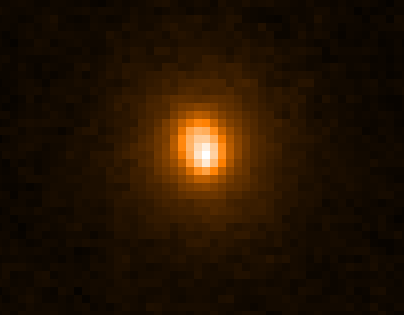
\includegraphics[width=0.8\linewidth]{Figure/NGC7213.png}\\
\caption{Image of NGC7213, one of the AGNs in the sample. Only the central groupings of pixels are dominated by AGN emission, the rest are dominated by stellar emission.}
\label{fig:NGC7213}
\end{figure}
\\
Due to the non-negligible nature of the stellar contribution towards the observed emission, it becomes necessary to separate the two components. This presents two separate challenges;
\begin{enumerate}
\item how to identify and locate the center of the AGN in the obtained image - so an astrometrical challenge
\item how to determine the angular size of the AGN in the observed image - so an aperture challenge
\end{enumerate}
following this challenge it became necessary to identify relevant stars for use as standard stars in the aim to create light curves independent of nightly observational conditions. In this regard it became an issue that the Pan-STARRS survey does not extend bellow a declination of $-30^\circ$, this necessitated the use of REM data to calibrate relevant southern Standard Stars in the g,r,i and z bands. 

\subsection{Finding the AGN}

\subsubsection{Astrometry of the AGN}
%The initial difficulty in any astronomical observations is locating the object of interest.
This project investigated two different approaches to locating the center of the AGN in the obtained REM images. Both appraches had their own individual strengths and shortfalls. The first approach relied on the use of the existing astrometrical calibration of the images, as done by the REM Telescope, or updating them later using a software like Pin-Point, or equivalent software. The second approach investigated is the use of the SEXtractor software. This software identifies abnormal pixel values in the image, based upon a search criteria and an underlying algorithm, that is neither the scope nor interest of this project. The SEXtractor software then return a list of pixel groupings fitting the search criteria, and knowing the approximate pixel location of the stellar object of interest it becomes possible to identify the center of this astronomical object. \\
Both methods had advantages and disadvantages. Utilising accurate astrometry, when applicable, is a fast mode of investigation both due to the use of broadcasting operations on numpy arrays, and due to the convenience of pre-identifying the correct object for investigation, as opposed to having to compile a list of all possible objects everywhere in the image. Additionally, assuming accurate geometry in the image, this method allows investigation of the center, as it is determined by larger surveys, of the AGN as opposed to attempting to find the spatial location of the SMBH in the AGN, and risk stellar noise combined with galactic inclination angle skewing the results. Conversely the same advantage is also the primary disadvantage of the accurate astrometry method of identifying the AGN in the obtained images. This method does not take into consideration the actual pixel configurations on the image, only the pixels that, according the the astrometry, is expected to be of relevance. This then leads to the risk, that in the case of non-perfect astrometry, the program may exclude some, or the entire light contribution from the AGN. This could be counteracted by using a larger aperture, but this has its own issues, as discussed later. \\
The second method investigated for use in this project utilises, as mentioned, the SEXtractor software. The main advantage of this method is that even in the case of slightly inaccurate, although not missing, astrometry, it is still possible to find the peak intensity of the observed astronomical objects. Thus this method allows for inaccurate astrometry on the obtained images, and thus theoretically allows the determination of the location of the AGN engine. The disadvantage in return is the significantly slower speed by which the light curves are generated, as well as the impact of noise, stellar light and inclination angle of the host galaxies to play in. \\
\\
\emph{Figures \ref{fig:Astrometry_NGC7213}} and \emph{\ref{fig:Astrometry_Tycho-22-1}} shows the difference between the expected location of the AGN of NGC3783 and the standard star Tycho-2 7740-22-1 respectively and the by SEXtractor determined locations. The errors observed in \emph{Figures \ref{fig:Astrometry_NGC7213}} and \emph{\ref{fig:Astrometry_Tycho-22-1}} are compounded by two sources of error that can be distinguished between. In the plot for Tycho-2 7740-22-1 it is observed that the difference between the expected location of the Standard Star and the, by SEXtractor, determined location coordinates, in the astrometrical calibration inherent in the images, is dispersed in a random circle, with no regards to time of observation, around the expected location. This must conceivably, should one assume that the located center of the Standard Star is not otherwise affected, give an accurate demonstration of the inaccuracy in the supplied astrometry. \emph{Figure \ref{fig:Astrometry_NGC7213}}, however, shows the location error associated with the AGN of NGC3783. In this case it is clear that the average SEXtractor locationis shifted away from the expected location, in addition to showing the same relative scatter. Thus, if one accepts the results from the point-like Tycho-2 7740-22-1 as an accurate estimation of the error in the astrometry, and the official location of the center of NGC3783, as determined by larger, more extensive surveys, then it must be clear that the SEXtractor softwareis not capable of accurately determining the center of the AGN based upon the peak intensity of the light emitted from NGC3783. This error likely arises based upon the inclination angle of the galaxy skewing the Point Spread Function of the entire galaxy by "hiding" some of the light from stars in the part of the galaxy "leaning away" from the line-of-sight. Thus the SEXtractor method might see the inclusion of excessive stellar light, however the astrometry accuracy method might lead to missing the AGN, and the Starndard Stars, either party or entirely. In this project the choice thus became the use of the SEXtractor software, as the astrometry precision method was deemed too unreliable, and the image quality was such that third party software, such as Pin-Point, designed to improve astrometry often either failed to provide significantly improved astrometry, or failed entirely. 

\begin{figure}[htp!]
\centering
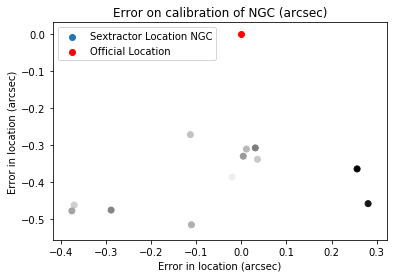
\includegraphics[width=0.7\linewidth]{Figure/Astrometry_NGC3783.png}\\
\caption{The Astrometric precision on the obtained images with respect to the center of the AGN NGC3783. The x-axis is the error in the Right Ascension and y-axis the error in Declination Angle, the lightening colour of the Sextractor Locations are in response to the time of observation, demonstrating a lack of relation in this regard.}
\label{fig:Astrometry_NGC7213}

\centering
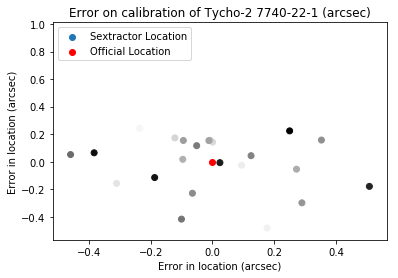
\includegraphics[width=0.7\linewidth]{Figure/Astrometry_Tycho-22-1.png}\\
\caption{The Astrometric precision on the obtained images with respect to the center of the standard star Tycho-2 7740-22-1. The x-axis is the error in the Right Ascension and y-axis the error in Declination Angle, the lightening colour of the Sextractor Locations are in response to the time of observation, demonstrating a lack of relation in this regard.}
\label{fig:Astrometry_Tycho-22-1}
\end{figure}

\subsubsection{Aperture Choice}
The aperture choice 

\subsection{Absolute Flux and Absolute Magnitude}
Identifying the absolute magnitude and flux of the observed AGN's necessitates the use of observed standard stars. Structure function observations made by Vries et al. 2004 shows the stellar Structure Functions to be flat, whereas AGN Structure Functions show a significant slope. This fits the known characteristics of stellar flux of being constant over long time-scales. This quality of stellar flux can be utilised in determining the absolute flux, and magnitudes of observed variable sources. \\
\\
Ground based astronomical observations does not demonstrate a constant observed flux on stellar objects as they are heavily influenced by various noise parameters associated with the earth atmosphere. This section will cover these noise parameters associated with the earth atmosphere, and describe the solution utilised in this project. \\
\subsubsection[Earth Atmosphere and associated uncertainties]{Earth Atmosphere and associated uncertainties\footnote{This section builds heavily on Léna, Lebrun \& Pelat, Observational Astrophysics, Third Edition.}}
The atmosphere of earth consists of different layers of varying temperature. These layers all have different impact upon the observations made. The different layers of the atmosphere is shown in (FIGURE 2.1 FROM OBS. AST. BOOK) and the temperature, altitude and pressure relations in (FIGURE 2.2 FROM OBS. AST. BOOK).\\
\\
Astronomic observations can be influenced by the earth atmosphere by either $total$ or $partial$ absorption. In the case of $partial$-absorption the atmosphere through which the observations are carried out alters the spectra of the observed sources. These changes are caused by $telluric\ absorption\ bands$ that can be identified, to avoid misinterpreting the spectra obtained. In the case of $total$-absorption it is possible to determine $transmission\ windows$ at any relevant altitude, and thus identify the altitude at which observations becomes impossible and thus the optical placement of the telescope based upon the local $transmission\ windows$ and the local $partial$-absorption. This project is not interested in the process behind the location of the relevant telescope. It is however necessary to understand the importance of the noise generated by the local conditions. In \emph{figure \ref{fig:poor_night} and \ref{fig:good_night}} atmospheric weather data for two nights are shown. These nights differs significantly in the air humidity and cloud coverage, and the changes in same over the course of the night. \\
\\
The Earth atmosphere is composed of several gases that influences the observed spectra of astronomical objects from ground based observations. The absorption spectra of several of these gases are demonstrated in \emph{figure \ref{fig:atmospheric_absorption}}.\\
\\
\paragraph[Water Vapour:]{Water Vapour:}\mbox{}\\
Water vapour in the atmosphere is highly dependent of altitude and local geographics. It is as shown in \emph{figure \ref{fig:atmospheric_absorption}} the cause for absorption over a great range of wavelenghts. The water vapour can be described by either the $humidity$, being the expression of the amount of water vapour as compared to the maximum possible water vapour at a given volume at the relevant temperature, or the $mixing\ ratio$. The $mixing\ ratio$ is an expression of the mass of water vapour in 1kg of air ($equation$ \ref{eq:mixing_ratio}) and is altitude dependent, 
\begin{equation}
r = \frac{m_{H_{2}O}}{m_{air}}
\label{eq:mixing_ratio}
\end{equation}\\
with r being the mixing ratio, that can vary between 0 and $r_{s}(T)$, the latter being the saturation mixing ratio, varying by altitude and temperature as shown in $figure$ \ref{fig:mixing_saturation_ratio}.
\begin{figure}[t!]
\center
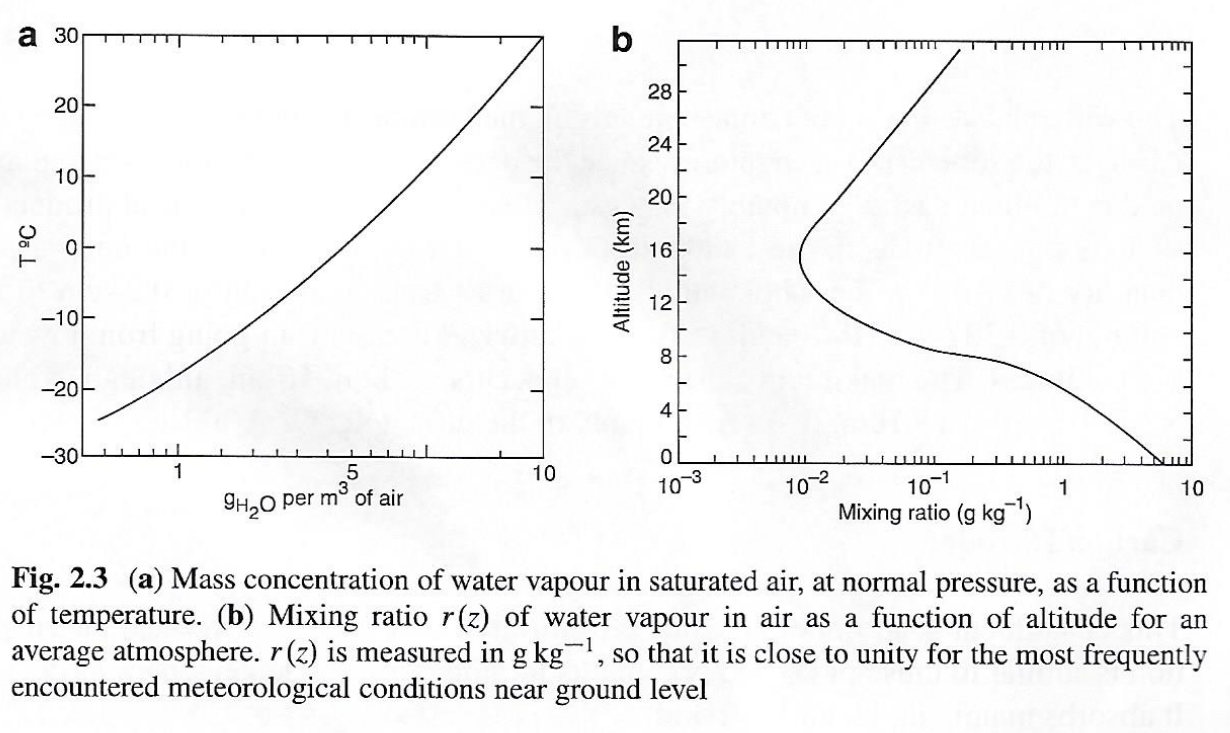
\includegraphics[width=1.\linewidth]{Figure/water_vapour.png}
\caption{Copy from Léna, Lebrun \& Pelat, Observational Astrophysics, Third Edition.}
\label{fig:mixing_saturation_ratio}
\end{figure}\\
\begin{figure}[t!]
\center
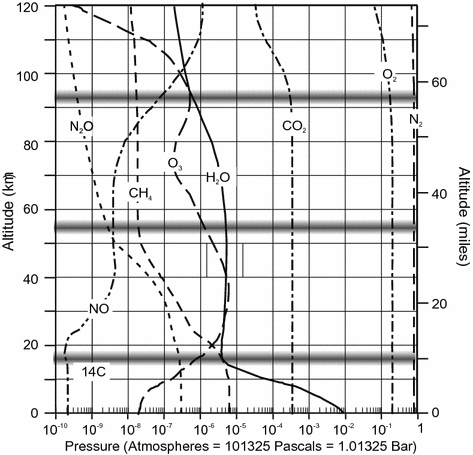
\includegraphics[width=.4\linewidth]{Figure/atmospheric_gases.png}
\caption{The contribution to the atmospheric pressure from various atmospheric gases. \\Copy from Hay W.W. (2013) The Atmosphere. In: Experimenting on a Small Planet. Springer, Berlin, Heidelberg.}
\label{fig:atmospheric_gases}
\end{figure}\\
\\
It is thus possible to determine the coloumn density of water vapour in the atmosphere through $equation$ \ref{eq:h_H2O},
\begin{equation}
h_{H_{2}O} [cm] = \rho_{0} [gcm^{-3}]\int_{z_{0}}^{\infty}r(z)e^{-z/H}dz,
\label{eq:h_H2O}
\end{equation}
with z being the altitude, $\rho_{0}$ being the density at $z=0$ and H being the scale height.\\
\\
Water vapour absorption arise from both \emph{pure rotational molecular transitions} and \emph{electronic molecular transitions} and this, combined with its distribution throughout the atmosphere, causes the varied absorption seen in \emph{figure \ref{fig:atmospheric_absorption}}. \\
\\
\paragraph{Ozone:}\mbox{} \\
The Ozone layer absorbs mainly in the ultraviolet range ($\lambda < 300 nm$) and is a very significant absorber in a narrow range of absorption as shown in \emph{figure \ref{fig:atmospheric_absorption}}. The highest concentration of ozone is at an altitude of $\sim16\ km$, as such it cannot be avoided in ground based observations. Ozone absorbs by \emph{pure rotational molecular transitions} and \emph{electronic molecular transitions}. The contribution towards the ozone pressure can be seen in $figure$ \ref{fig:atmospheric_gases}. \\
\\
\paragraph{$CO_{2}$:}\mbox{} \\  
With a constant mixing ration, independent of altitude ($figure$ \ref{fig:atmospheric_gases}.), $CO_{2}$ is an important source of infrared absorption, particularly mid-IR, in the atmosphere. $CO_{2}$ absorbs through \emph{pure rotational molecular transitions} and \emph{rotational-vibrational molecular transitions}

\begin{figure}[t!]
\center
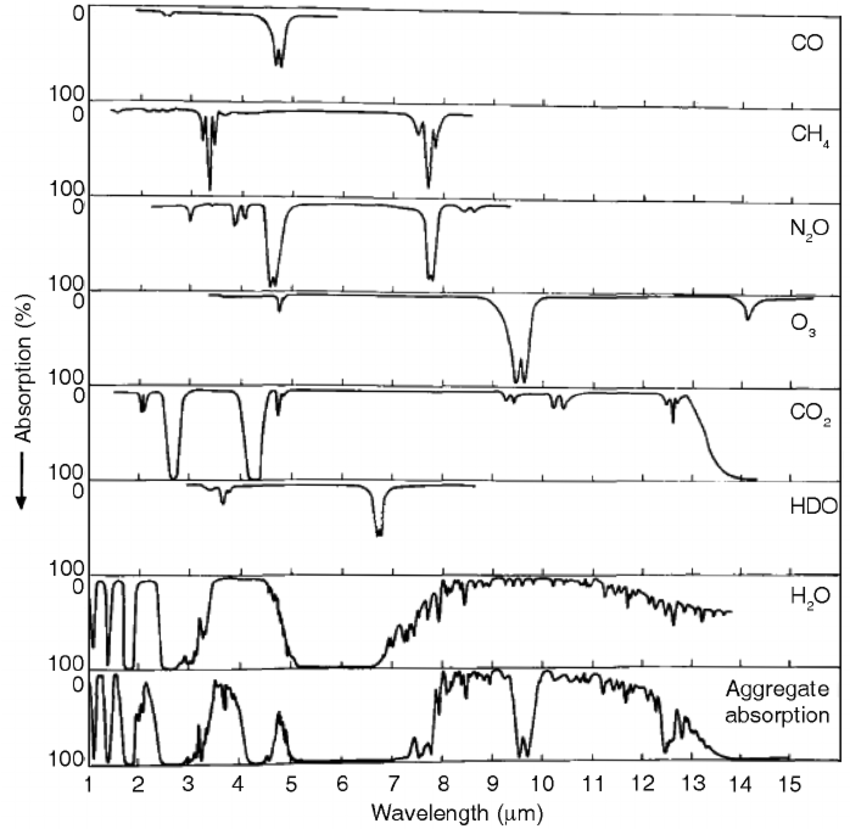
\includegraphics[width=0.7\linewidth]{Figure/Infrared-absorption-spectra-for-various-atmospheric-gases.png}
\caption{The absorption features of various absorbing gases in the Earth atmosphere. Brunetti and Prodi 2015}
\label{fig:atmospheric_absorption}
\end{figure}

\subsubsection[Magnitude:]{Magnitude:\footnote{This section builds heavily on Schneider 2006}}
\emph{Apparent magnitude:} \\
The magnitude scale is a logarithmic flux scale utilised to compare luminosities between seperate astronomical objects. It was implemented prior to the invention of precision measurement tools utilised for accurate flux measurements. The logarithmic nature of this scale originates in the human eye, as the human eye ability to identify differing light intensities is not linear, rather it scales roughly logarithmically. This original measuring scale was based upon the observed differences between astronomical object, independent on distance and is called \emph{apparent magnitude}. The magnitude scale is for historical purposes, due to the inherent historical difficulty in observing outside the optical spectrum, only used in optical astronomy. It has however been modified with a more precise modern definition (\emph{equation \ref{eq:app_mag}}) 
\begin{equation}
m_{1} - m_{2} = -2.5log(\frac{F_{1}}{F_{2}}),
\label{eq:app_mag}
\end{equation}
with $m_{1}$ and $m_{1}$ being the \emph{apparent magnitudes} of the astronomical objects $1$ and $2$ and $F_{1}$ and $F_{2}$ the fluxes of same. The constant 2.5 is chosen as to achieve the closest agreement between the historically based visual magnitudes and the moder precision based magnitude system. \\
\\
As demonstrated in \emph{figure \ref{fig:atmospheric_absorption}} the flux observed in ground based observations are heavily influenced by the wavelengths bands chosen for observation as well as the differing energy spectral distributions vary between objects. As such a series of filters are designed with magnitudes defined for all relevant observational filters. In this project the filters of note are the SDSS filters g,r,i, and z and the Johnson-Cousins filters J,H and K as shown in \emph{figure \ref{fig:filters}}. \\
\\Magnitudes are thus filter dependent and the denotation for the magnitude in filter K is $m_{K}=K$. In order to determine the relationship between the magnitudes measured in different filters, and have a comparison table between astronomical objects a zero magnitude star is chosen, the type A0 star with Vega as the normal example. In this Vega system $U=B=V=R=I=J=H=K...=0$. The alternative to the Vega system is the AB system for apparent magnitudes. In this system it is assumed that the zero magnitude definition for all filters is not the SED of an actual star, but rather the constant flux in all bands of $F=2.89\times10^{-21}erg\ s^{-1}cm^{-2}Hz^{-1}$. The conversion between AB and Vega magnitudes are demonstrated in \emph{table \ref{tab:Vega_AB_conversion}}.\\
\begin{wraptable}{l}{5.5cm}
\caption[The differences between the AB zero magnitudes and the Vega zero magnitudes in the filters used by this project]{The differences between the AB zero magnitudes and the Vega zero magnitudes in the filters used by this project.\footnote{http://www.astronomy.ohio-state.edu/~martini/usefuldata.html}}
\begin{tabular}{|l|l|}
\hline
$Filter$ & $m_{AB}-m_{Vega}$ \\
\hline
\hline
$g$ & -0.08 \\
\hline
$r$ & 0.16 \\
\hline
$i$ & 0.37 \\
\hline
$z$ & 0.54 \\
\hline
$J$ & 0.91 \\
\hline
$H$ & 1.39 \\
\hline
$K_{s}$ & 1.85 \\
\hline
\end{tabular}
\label{tab:Vega_AB_conversion}
\end{wraptable}
\\
\emph{Absolute magnitude:} \\
The apparent magnitude discussed so far is an interpretation of the strength of the flux observed, and not a representation of the luminosities of the objects observed. The apparent magnitude does not consider the distance ($D$) of the observed objects. To overcome this short-coming the absolute magnitude is used. For an isotropically emitting source of distance $D$ and luminosity $L$ the flux $F$ is found by \emph{equation \ref{eq:FDL}}
\begin{equation}
F = \frac{L}{4\pi D}.
\label{eq:FDL}
\end{equation}
In the same manner that the \emph{apparent magnitude (m)} is an interpretation of the observed flux $F$, the \emph{absolute magnitude (M)} becomes an expression for the luminosity $L$. The absolute magnitude is defined to be the apparent magnitude in the case of the emitter being located at a distance of $10\ pc$ and the relationship is given by \emph{equation \ref{eq:absolute_magnitude_relationship}}
\begin{equation}
m - M = 5log(\frac{D}{1\ pc}) - 5 \equiv \mu,
\label{eq:absolute_magnitude_relationship}
\end{equation}
with $\mu$ being the \emph{distance modulus}, and thus a logarithmic measure of the distance to the source. \\
\\
\emph{Bolometric magnitudes:} \\
The \emph{apparent bolometric magnitude} ($m_{bol}$) is the magnitude of a light emitting source calculated from the flux integrated over all wavelengths 
\begin{equation}
m_{bol} = -2.5log(F) + const.,
\label{eq:m_bol}
\end{equation}
with the constant being calculated based upon reference stars. The \emph{absolute bolometric magnitude} ($M_{bol}$) is identical to the \emph{apparent bolometric magnitude} just based upon the luminosity integrated over all frequencies. 

\subsubsection{Flux:}
Flux is the energy received on a given area over a given time-frame. The flux observed by a telescope is dependent upon the luminosity of the source and the distance between source and observer (see \emph{equation \ref{eq:FDL}}) as well as, in the case of ground based observations, the atmospheric conditions at the time and location of the observation. As such the measured flux by the telescope is not in itself an indication of the energy output by the emitter, nor the change in energy output from the emitter, the former being distance and atmospheric dependent, and the latter dependent upon the atmospheric conditions. These problems necessitates calibration of all observations against known emitters. \\
\\
Flux calibration of energy varying emitters can be done based upon simultaneous observations of non-energy varying emitters. One such emitter is stars, as stellar light sources has almost flat structure functions and power spectra (discussed later) over periods of human time-scales, objects with these characteristics is henceforth named \emph{standard stars}. Thus it becomes possible to calculate the flux of the observed AGNs based upon the observed flux of simultaneously sampled standard stars at small angular separations. \\
\\
Nightly measurements of the flux of standard stars based on space based telescopes will demonstrate a constant measured flux (baring exo-planetary transits etc.). Ground based observations however will vary dependent on humidity, cloud coverage etc., it is however possible to negate this issue by comparing the observed objects with known standard stars. \\
\\
Flux calibration done this way lends much of its derivation to the previous discussion of \emph{apparent magnitude}. The apparent magnitude calculation is dependent upon the observed fluxes of two objects observed under identical conditions, while knowing the expected magnitude of one of them. In the case of this project the known quantity is a standard star, with a magnitude determination made by a larger survey, such as SDSS, PanSTARRS etc. Through \emph{equation \ref{eq:apparent_magnitude}} it is thus possible to calculate the expected flux of a varying object through the AB magnitude system flux zero point of $F_{m_{AB}=0}=2.89\times10^{-21}erg\ s^{-1}cm^{-2}Hz^{-1}$. It is however of note that the two observed objects inevitably will have different angles on the night sky, and therefore dependent on the WRITE ABOUT AIR MAG HERE!!!!!!!!!!!!!!!!!!!!!!!!!!!!!!!!!!!!!!!!!!!!!!!!!!!!!!!!!!

\begin{figure}[t!]
\centering
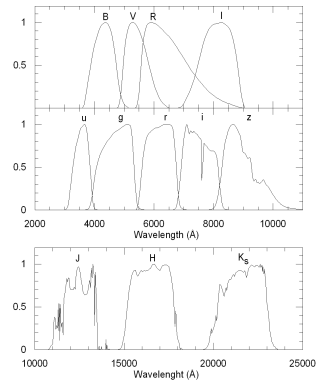
\includegraphics[width=0.5\linewidth]{Figure/filters.png}
\caption{The filters used in this project. The SDSS filters g,r,i and z and the Johnson-Cousins J,H and K filters. Figure from Bilir et al. 2007.}
\label{fig:filters}
\end{figure}

%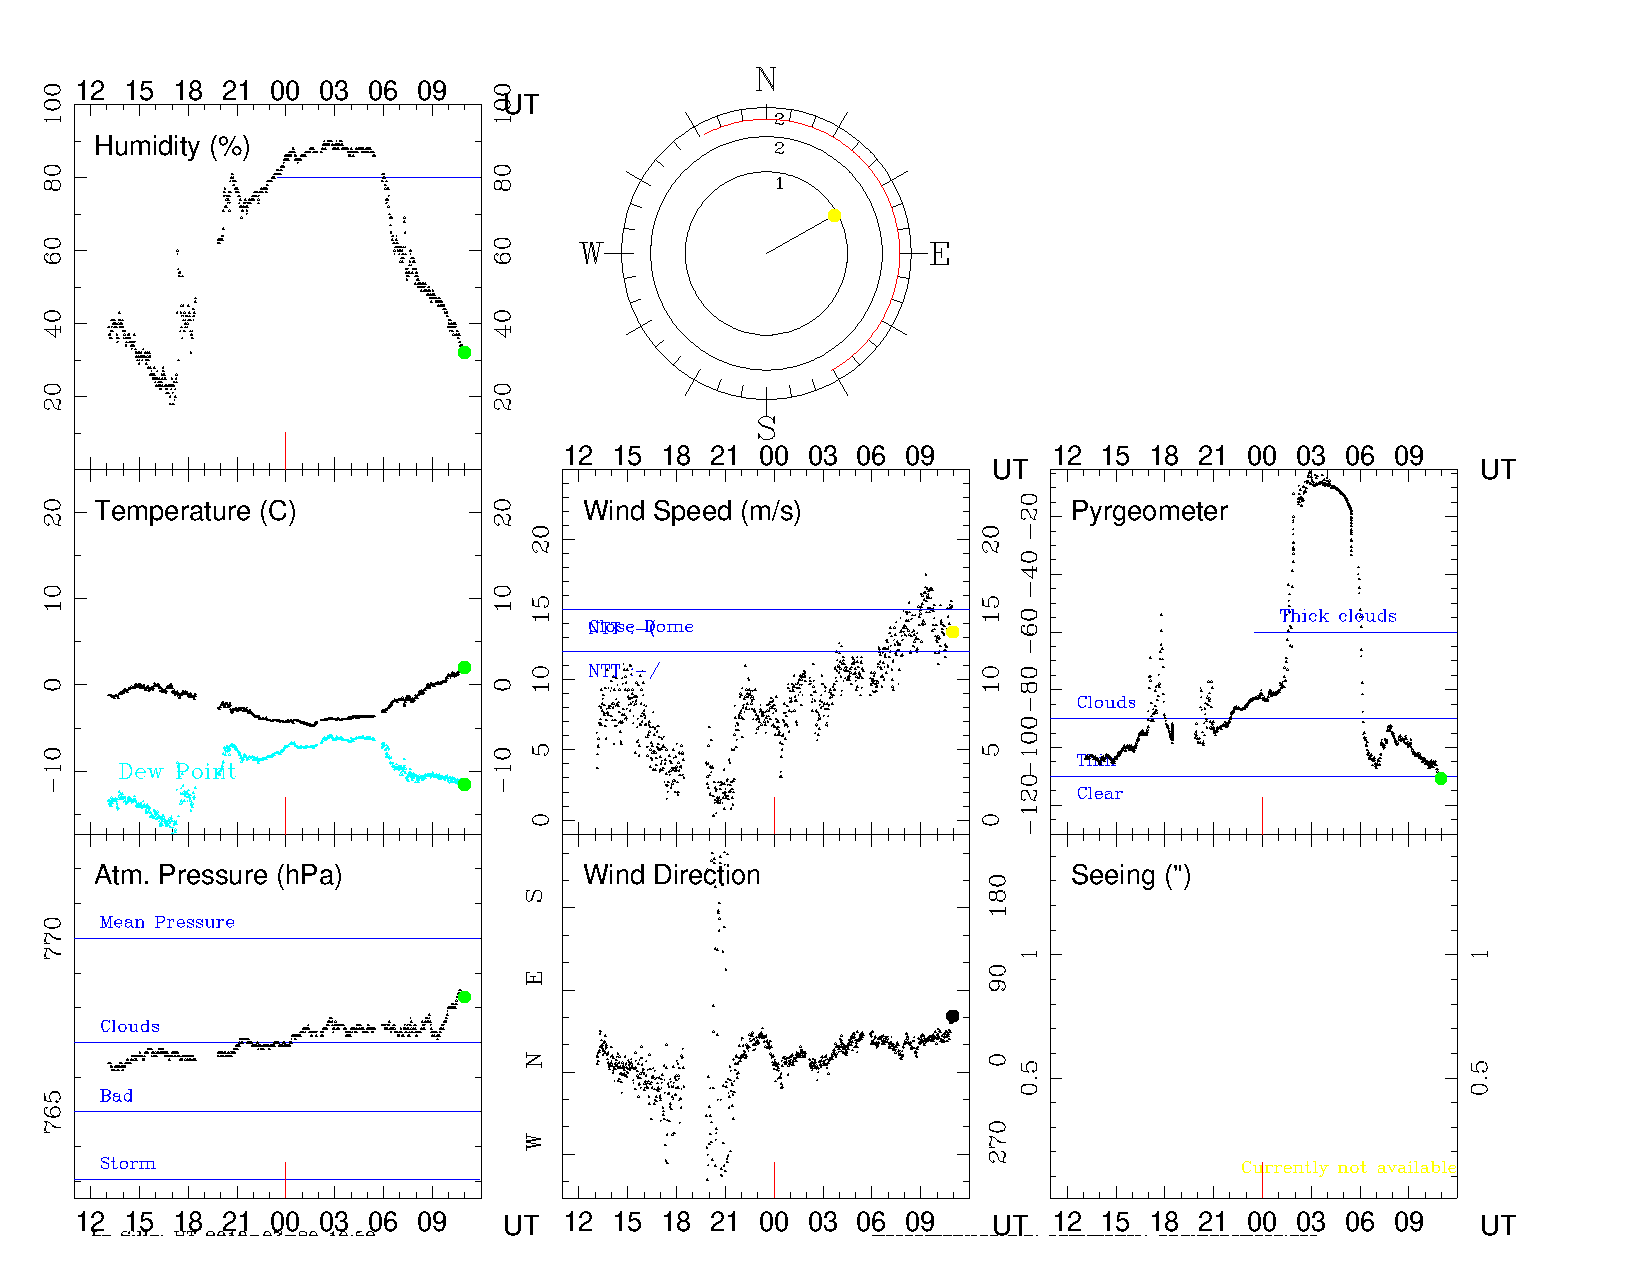
\includepdf[pages=-]{Figure/end180720.pdf}
\begin{figure}[htp!]
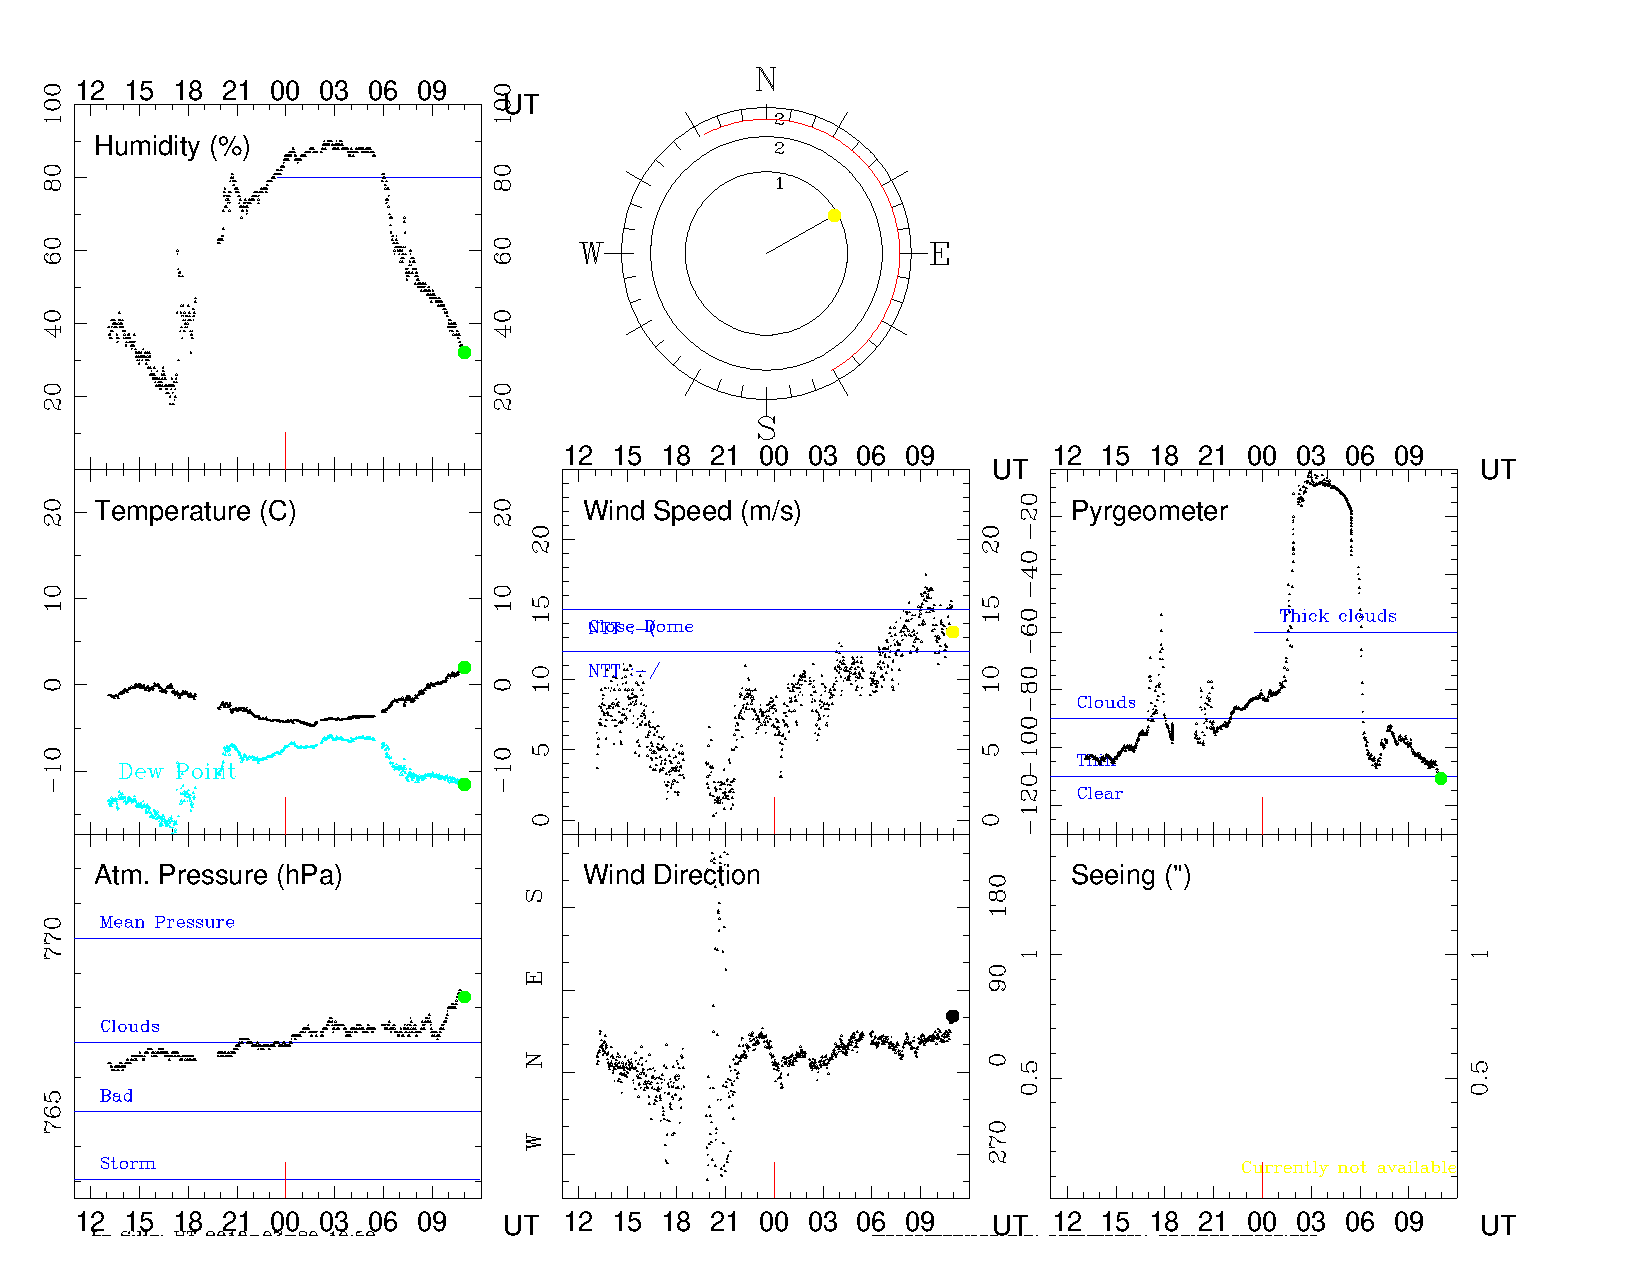
\includegraphics[width=1.1\linewidth]{Figure/end180720.pdf}
\caption{Atmospheric data for the La Silla Observatory Site in Chile at the night of 20th July 2018. This night demonstrates significant and varying cloud coverage of the observatory site as well as significant and changing humidity. At this night comparing observations obtained at midnight and 03.00 should not be compared, due to the significant difference in the cloud coverage influencing the results. Data from the La Silla - Meteominitor.}
\label{fig:poor_night}
\end{figure}

\begin{figure}[htp!]
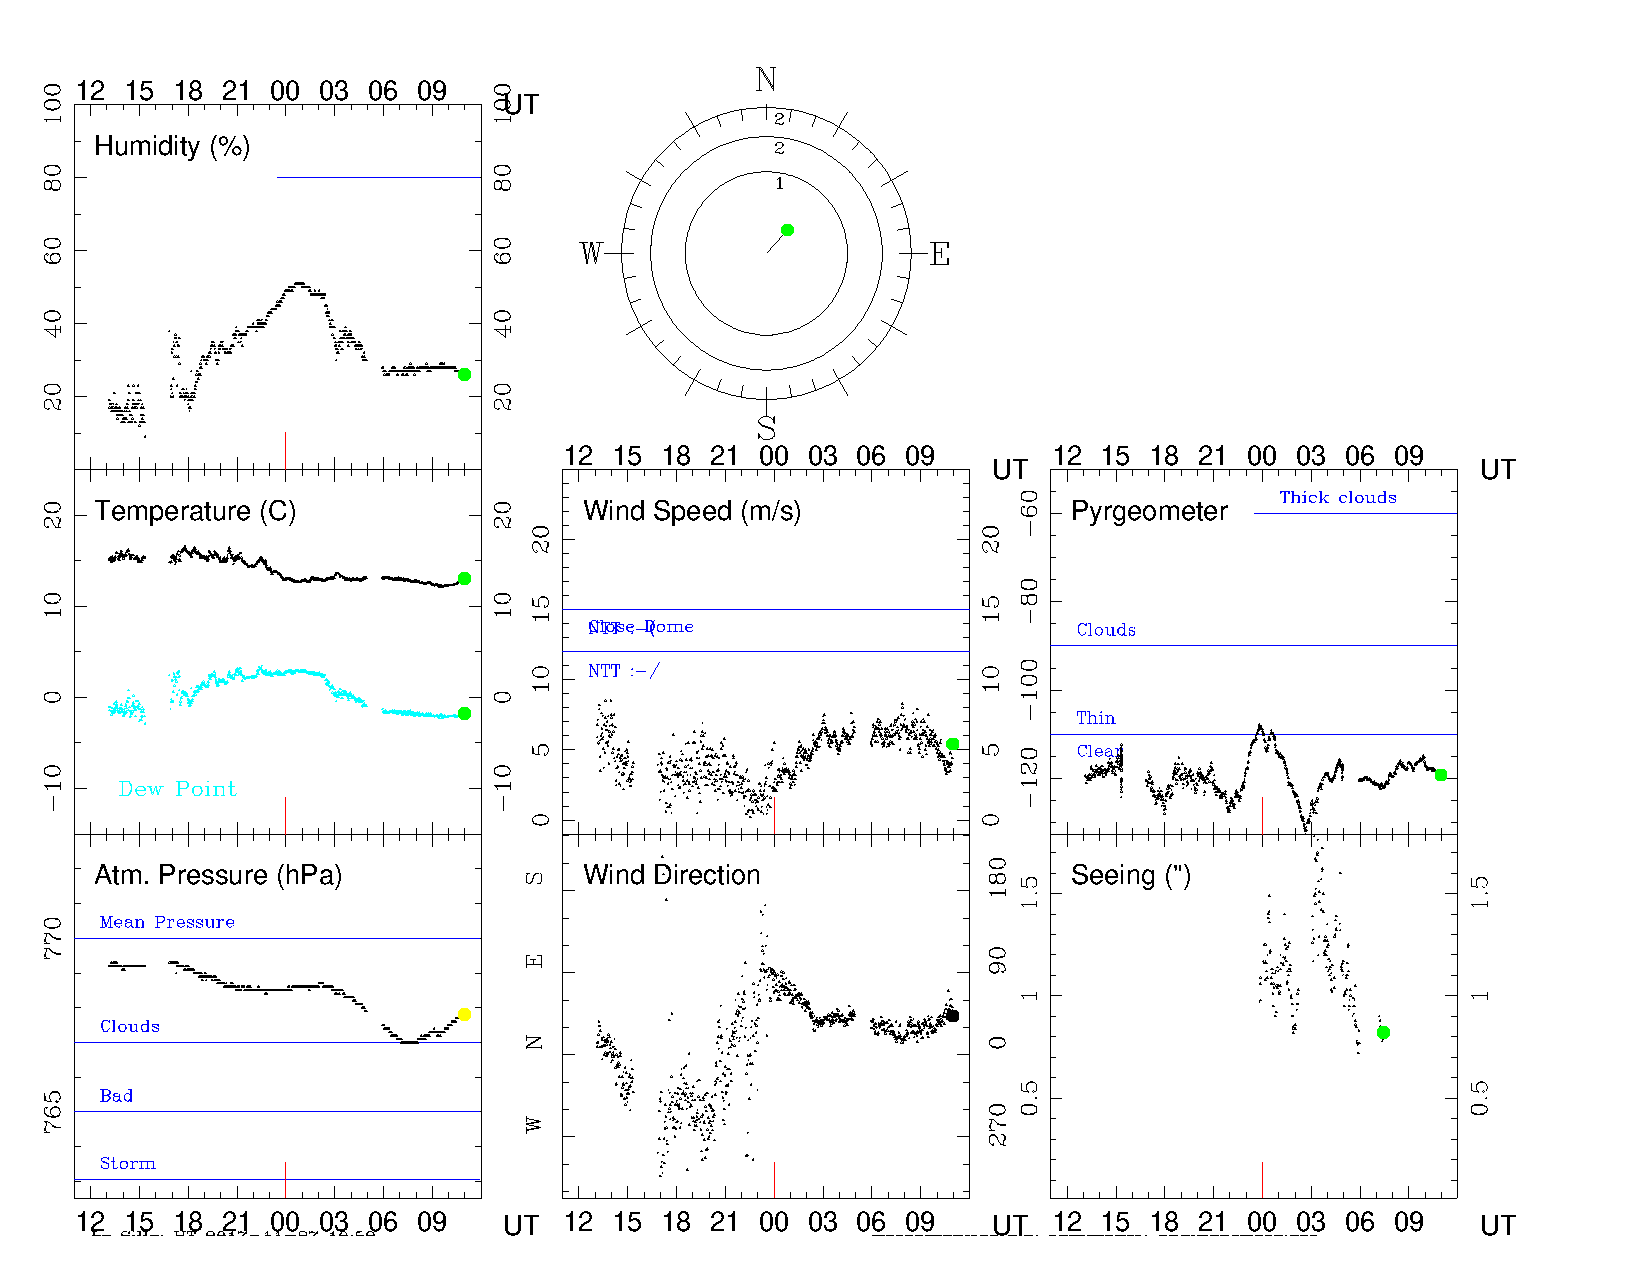
\includegraphics[width=1.1\linewidth]{Figure/end171127.pdf}
\caption{Atmospheric data for the La Silla Observatory Site in Chile at the night of 27th November 2017. This night demonstrates lower and more constant cloud coverage of the observatory site as well as lower but changing humidity. This night will be a significantly improved night to compare observations of different astronomical objects at different parts of the night sky. Data from the La Silla - Meteominitor.}
\label{fig:good_night}
\end{figure}

\subsection{Error in Fluxes}
Astronomical observations are subject to observational uncertainties. These uncertainties arises through atmospheric disturbances, as previously discussed, as well as interstellar and intergalactic material blocking part, or entire, emission lines thus skewing the observed data. In this project astronomical disturbances, beyond those inherent in the AGN structure, is of little actual interest. It is essentially assumed that the AGN is sufficiently close as to ignore the intergalactic material, or that the influence of same would be evenly distributed across all observed bands. Seyfert Galaxies are inherently disk galaxies and as the observed AGNs are Type I Seyferts and as such the BLR is visible. It must this stands to reason that the Galaxies is observed head-on and as such the contribution from the ISM is lessened. (ASK SUPERVISOR!!!!!!!!!!!!!!!!!!!!!!)\\
\\
The flux based error of interest in this project is the \emph{signal-to-noise ratio (S/N)}. The \emph{signal-to-noise ratio} is a measure of the relative strength of the noise in the observation in relation to the signal strength. 

\section{Finding Continuum}
In this section the process utilised in determining the used continuum destribution of the observed quasar data is described. The method used was found through a combination of reading relevant literature and implementation of numerical MCMC algorithm. At no point in this endeavor has the aim been to find the absolute Continuum Light Curve (driving function). The objectively correct driving function is of no real importance in the investigation, and therefore would cause unnecessary time to pursue. The difficulty in determining the absolute driving function is in the lack of knowledge of the actual band dependent transfer function of the observed Light Curves (LC). Additionally the interest in the project is the timelag between the observable bands, and as such the relative transfer functions as opposed the the absolute transfer functions. \\
This section will be focused upon describing the methods used and the reasons behind the decisions taken.\\

\section{Defining a Light Curve}
Three main methods of characterising Light Curves has been explored during the course of this project. Each methods have their own advantages and disadvantages, and to accurately formulate a working model for the continuum Light Curve all three has been utilised. The methods are;
\begin{enumerate}
\item The Stochastic model described in Kelly et al. (2009). This model builds on the assumption of AGN variability being described as a \emph{Continuous Time First-Order Autoregressive Process} (\emph{CAR(1)}).
\item Modeling the AGN variability as a Power Spectrum with Power Spectral Density slope of $\alpha=-2.3...-3.4$.
\item Using Structure Functions to analyse AGN variability.
\end{enumerate}
These three approaches allows for the identification and evolution of different aspects of AGN light curves. The Structure Function allows for the understanding of certain key characteristics of the observed and modeled Light-Curves, whereas both the Kelly et al. (2009) and the Power Spectrum approach allows for the modeling and evolution of AGN 

\subsection{Original Data Material and Kelly manipulations} \label{Kelly}
Light Curve sampling is dependent on atmospheric conditions, the visible night sky and observation time on the telescope. As such observed light-curves will often be unevenly sampled with time intervals of days or perhaps weeks. As such a method of modeling the missing data can be necessary, it is with this aim that the Kelly et al. (2009) described Stochastic model (from here named \emph{"Kelly model"}) is investigated. In the data obtained for the purpose of this project considerable and uneven time intervals presents itself. The Kelly model is a model build over the assumption that a Light-Curve observed in an AGN can be modeled as a \emph{Continuous Time First-Order Autoregressive} (\emph{CAR(1)}) \emph{Process}. The Kelly model is consistent with a power spectra of the form $P(f)=1/f^{2}$, this as described later, despite being a common assumption for AGN variability, is not an entirely accurate representation of the observed AGN variability, thus the Kelly model cannot, standalone, define an actual AGN Light-Curve without additional development. \\
\\
The Kelly model is, as mentioned, a Continuous Stochastic model, rather than modeling Liht-Curves using Fourier (Spectral) techniques. It is modeled as Continuous time as the physical processes occurring in the accretion disk is continuous and it provides a natural way of handling irregular sampling. The model uses 3 different parameters to define the Light-Curve created;
\begin{enumerate}
\item A characteristic time-scale, called the \emph{"relaxation time"} ($\tau_{Kelly}$)
\item Amplitude of short time-scale variability
\item Mean value of the Light-Curve
\end{enumerate}
The \emph{"relaxation time"} is given as the time-scale at which the time series becomes uncorrelated and is easily associated with the various characteristic time-scales inherent in the accretion disk physics such as the light crossing time, the orbital time-scale and the thermal time-scale.
\begin{equation}
t_{lc} = 1.1\times(\frac{M_{BH}}{10^{8}M_{O}})(\frac{R}{100R_{S}})~days
\label{eq:t_lc}
\end{equation} 
\begin{equation}
t_{lc} = 104\times(\frac{M_{BH}}{10^{8}M_{O}})(\frac{R}{100R_{S}})^{3/2}~days
\label{eq:t_orb}
\end{equation} 
\begin{equation}
t_{lc} = 4.6\times(\frac{\alpha}{0.01})^{-1}(\frac{M_{BH}}{10^{8}M_{O}})(\frac{R}{100R_{S}})^{3/2}~yr
\label{eq:t_th}
\end{equation} 
In Kelly et al. 2009 the relationship between the Characteristic time-scales in \emph{equations \ref{eq:t_lc}, \ref{eq:t_orb} and \ref{eq:t_th}} and the \emph{relaxation time} is investigated. They conclude that although both the $t_{orb}$ and the $t_{th}$ provides reasonable fits, the best fit is the thermal time-scale. The differential equation governing the $Kelly \ model$ is given through $equation$ \ref{eq:Kelly2009}.   

%The Kelly model builds on previous works identifying the Power Spectral Density Slope to be $\alpha \sim -2$, and inaccurate assumption as later described, 


%The driving function is found based upon the observed light curves of the K-band. The REM data is observed in the KHJgriz bands. The REM data is uneven in the sampling and subject to several observation gaps of a 50 - 100 day period. Due to this sampling it has proved of interest to attempt to simulate the Observed Light Curves (observed light curve) across the observational gaps. These has been filled through the use of the Kelly Function (Kelly et al. 2009). The Kelly Function is not actually a function as much as a way of approximating the next point of the LC based upon the overall distribution of observed values. It is given by \emph{equation \ref{eq:Kelly2009}},

\begin{equation}
dX(t) = -\frac{1}{\tau_{Kelly}}X(t)dt + \sigma\sqrt{dt}\epsilon(t) + bdt
\label{eq:Kelly2009}
\end{equation}
with $b\tau_{Kelly}$ being the observed mean value of the observed light curve and $\tau_{Kelly}$ is the relaxation time additionally the variance on the Light-Curve is given by $\tau\sigma^{2}/2$. Additionally the $\epsilon(t)$ a white noise function of zero mean and variance of one, and $X(t)$ represents the Light-Curve. The Kelly approach introduces a slight shifting on the axis dependent on the direction of evolution and the direction in which the Light-Curve is read. Due to this bias in the $Kelly \ model$ it has been chosen during the course of this project to generate the \emph{Kelly Light-Curve} from both directions and use the mean Light-curve. This is examplified in \emph{figure \ref{fig:NGC3783K-Kelly}}

\begin{figure}[t!]
\centering
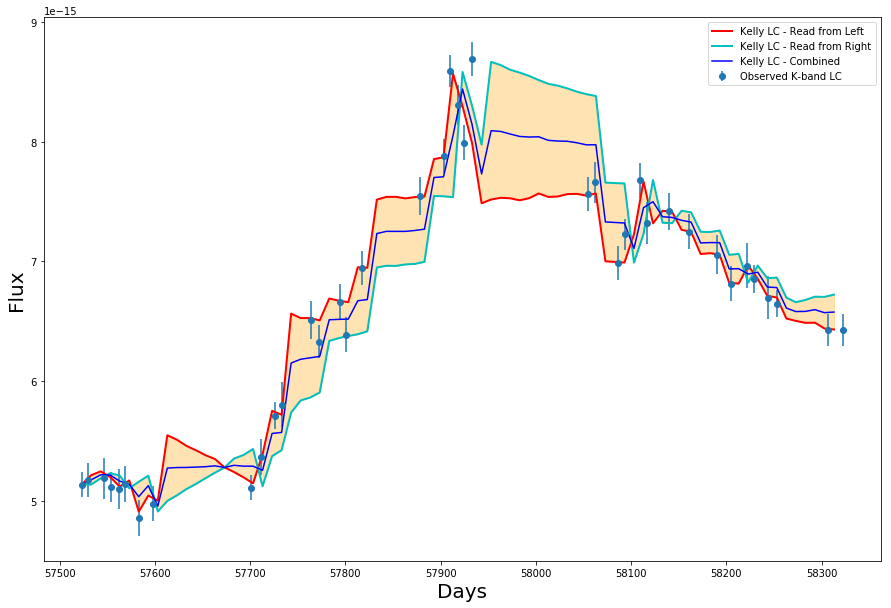
\includegraphics[width=1\linewidth]{Figure/NGC3783K-Kelly.png}\\
\caption{The Kelly function applied to the NGC3783 K-band spectrum. The red curve is the $Kelly \ method$ interpretation as applied from left to right, and the green is the opposing direction. It becomes apparent that significant bias can be found in the Kelly method as only applied in one direction.}
\label{fig:NGC3783K-Kelly}
\end{figure}

\noindent The three parameters defining the $Kelly \ model$ can be determined through the use of a maximum likelihood estimate from \emph{equations \ref{eq:p(b,sigma,tau)} through \ref{eq:a_i}}.
\begin{equation}
p(x_{1},...,x_{n}|b,\sigma,\tau) = \prod_{\mathclap{i=1}}^{\mathclap{n}}[2\pi(\Omega_{i}+\sigma_{i}^{2})]^{-1/2}\times exp[-\frac{1}{2}\frac{(\hat{x}_{i}-x_{i}^{*})^{2}}{\Omega_{i}+\sigma^{2}}]
\label{eq:p(b,sigma,tau)}
\end{equation}
\begin{equation}
x_{i}^{*} = x_{i}-b\tau_{Kelly}
\label{eq:x_star}
\end{equation} 
\begin{equation}
\hat{x}_{1} = 0
\label{eq:x_hat_1}
\end{equation} 
\begin{equation}
\Omega_{1} = \frac{\tau_{Kelly}\sigma^{2}}{2}
\label{eq:Omega_1}
\end{equation}
\begin{equation}
\hat{x}_{i>1} = a_{i}\hat{x}_{i-1}+\frac{a_{i}\Omega_{i-1}}{\Omega_{i-1}+\sigma_{i-1}^{2}}(x_{i-1}^{*}-\hat{x}_{i-1})
\label{eq:x_hat_i}
\end{equation}
\begin{equation}
\Omega_{i>1} = \Omega_{1}(1-a_{i}^{2})+a_{i}^{2}\Omega_{i-1}(1-\frac{\Omega_{i-1}}{\Omega_{i-1}+\sigma_{i-1}^{2}})
\label{eq:Omega_i}
\end{equation}
\begin{equation}
a_{i>1} = exp[-\frac{t_{i}-t_{i-1}}{\tau_{Kelly}}]
\label{eq:a_i}
\end{equation}
The $Kelly \ method$ as a $CAR(1)$ process has a power spectrum given by $equation \ ref{eq:Kelly_power_spectrum}$
\begin{equation}
P(f) = \frac{2\sigma^{2}\tau_{Kelly}^{2}}{1+(2\pi\tau_{Kelly}f)^{2}}
\label{eq:Kelly_power_spectrum}
\end{equation}
allowing the resulting Light-Curve to be separated in two different regimes. In the case of time-scales being short as compared to the $relaxation \ time$ the power spectrum falls as $1/f^{2}$ and in the case of time-scales longer than the $relaxation \ time$ the power spectrum becomes constant.  \\
\\
Analysing $figure$ \ref{fig:Kelly2009} one can identify one of the key weaknesses in the $Kelly \ method$ in the significant time-gaps displayed. The Kelly Function provides a generally reasonable fit in areas of reasonable coverage for the observations, however it proves unable to successfully predict reasonable suggested data for time-gaps of significant size. As such utilising the range of suggestions provided by the twin interpretations from opposing sides becomes useful. It may be possible to adjust this somewhat by introducing a dependence of time from the points of observation that the estimate is based upon. This however is not the focus at this time. 

\subsection{Power Spectral Density}' \label{PSD}
The Power Spectral Density (PSD) is an expression of variability in a function as a function of temporal frequency. The PSD is determined by calculating a periodogram (\emph{equations \ref{eq:zero_freq}, \ref{eq:mod_squared_Fourier} and \ref{eq:Power_Spectra}}). The $periodogram$ resultant of calculating the Power Spectral Density of real observable data is an $inconsistent$ estimator of the PSD, as the scatter observed in the periodogram is not decreasing as the number of observations is increased, necessitating averaging the periodogram. This can be done by either binning the calculated frequencies, or averaging over data segments, thus allowing an averaged periodogram to become a $consistent$ estimator of the PSD (Vaughan et al. 2003) \\
\\
In the case of AGN Light-Curves the interesting aspect of the PSDs becomes the slope of the $consistent$ estimator. This PSD slope (denoted $\alpha$) can be an indication of the time-dependent variability of AGN Light-Curves should a general tendency be identified. It is important to acknowledge that AGNs vary and as such, despite early assumptions of $\alpha=2$ the PSD slope is not identical across observed AGNs.\\
\\
The PSD can be obtained from both evenly and unevenly sampled light-curves. To calculate the PSD from a discrete Light-Curve ($X(t_{i})$) with N observed data points it is necessary to remove the zero-frequency power, by subtracting the mean from the Light-Curve,
\begin{equation}
X_{PSD}(t_{i}) = X(t_{i}) - \mu(X(t_{i}))
\label{eq:zero_freq}
\end{equation} 
and calculate the modulus squared of the discrete Fourier transform
\begin{equation}
|F_{N}(\nu)|^{2} = [\sum_{{i=1}}^{N}X_{PSD}(t_{i})cos(2\pi\nu t_{i})]^{2} + [\sum_{{i=1}}^{N}X_{PSD}(t_{i})sin(2\pi\nu t_{i})]^{2}
\label{eq:mod_squared_Fourier}
\end{equation} 
with $\nu$ being the sampled frequencies of the discrete Fourier transform occuring at evenly spaced intervals at $\nu_{min}$, $2\nu_{min}$, $3\nu_{min}$,...,$\nu_{Nyq}$, with $\nu_{min} = T^{-1}$ (T being total length of Light-Curve) and $\nu_{Nyq}$ being the Nyquist frequency of $(2T/N)^{-1}$. The power of the relevant function is obtained by nomalising $|F_{N}(\nu)|^{2}$ (Uttley et al. 2001)
\begin{equation}
P(\nu) = \frac{2T}{\mu^{2}N^{2}}|F_{N}(\nu)|^{2}.
\label{eq:Power_Spectra}
\end{equation} 
This Power Spectra allows the integration of the Power Spectra over a range $\nu_{1}$ to $\nu_{2}$ to determine the contribution to the fractional rms squared variability ($\sigma^{2}/\mu^{2}$) of the Light-Curve generated by variations on the time-scale $T_{2}$ to $T_{1}$. (FIND AND CHECK van der Klis 1997). The total fractional rms variability observed is thus determined by the square root of the integrated power spectrum. It is observed in Uttley et al. 2001 that the actually observed power spectra for AGN demonstrate either a Knee Model power spectra, by flattening to a slope of $\alpha=0$ at low frequencies or a high-frequency break model (by flattening to a slope of $\alpha=1$ at low frequencies). \\
The PSD slope is obtained through linear fitting in loglog-space past the "Knee" or "Break". \\
\\
In a study by Smith et al. 2018 of 21 Type I AGN Light-Curves from Kepler the PSD slopes has been studied. The AGNs studied by Smith et al. 2018 are comparable to AGNs studied in this project, in them being of the local universe, all but one of them with redshift $z<1$. In the study it is determined that the PSD slope ($\alpha$) ranges from -1.7 to -3.4 with a mean value of $\alpha_{mean}=-2.51$ and standard deviation of $\alpha_{std}=0.42$. This allows for better indications of the Physical relevance of the generated driving function of the observed AGNs, that is attempted in this project. 


\subsection{Structure Function} \label{Structure_Function}
The structure function is used to understand the behavior of long-term AN variability. Short-term AGN variability is generally accepted to be attributed towards relativistic beaming effects (READ UP ON THIS AND WRITE EXPLANATION FOR THIS IN THEORY), however long-term AGN variability is more difficult to ascertain the cause of. Suggestions towards possible causes is (as given in Vries et al. 2004 and Kawaguchi et al. 1998):
\begin{enumerate}
\item Disk Instability (described in Starling et al. 2004 READ UP ON IT AND WRITE HERE)
\item Super Novae event bursts close to the AGN 
\item Source extrinsic variations due to microlensing events along line-of-sight
\end{enumerate}
The structure function, as described by Kawaguchi et al. (1998) and Simonetti et al. (1985) (FIND THIS PAPER), is given by $equation$ \ref{eq:structure_function}
\begin{equation}
V(\tau) = \frac{1}{N(\tau)}\sum_{\mathclap{i<j}}[m_{opt}(t_{i})-m_{opt}(t_{j})]^{2}
\label{eq:structure_function}
\end{equation}
with $m_{opt}(t_{i})$ being the optical magnitude at the time $t_{i}$, $\tau$ being the time-difference $t_{i}-t_{j}$ and $N(\tau)$ being number of pairs of $\tau = t_{i}-t_{j}$. The structure function itself applied to an observed AGN Light-Curve will demonstrate three regimes (Kawaguchi et al. 1998, Hughes et al. 1992 (FIND THIS PAPER AND CONFIRM));
\begin{enumerate}
\item A plateau at time-lags exceeding the longest correlation time-scale, with a value twice the variance of fluctuations in the measurements 
\item Plateau at short time-lags with value twice the measurement noise (not in models without arbitrary measurement noise)
\item Power-law increase with time-lag as $[V(\tau)]^{1/2}\propto \tau^{\beta}$ between the two plateau'
\end{enumerate}
Additionally there is a comparability between the PSD slope ($\alpha$), discussed previously, and the structure function slope ($\beta$) of $\alpha=1+2\beta$ assuming $1\le\alpha\le3$ (FIND REFERENCE EITHER KAWAGUCHI OR VRIES).

\subsection{Transfer Functions}
In order to determine the driving function one must have an understanding of how the LC behaves from the Quasar to the observation. If one were to determine the exact Transfer Function at all times, it would then be possible to determine the exact driving function. However the transfer function is an unknown quantity and as the observed light curve is the result of the transfer function and the observed light curve (\emph{equation \ref{eq:OLC}}) (Andreas Skielboe 2016)
\begin{equation}
F_l(t,\lambda) = \int_{-\infty}^{\infty}\Psi(\tau,\lambda)F_C(t-\tau)d\tau
\label{eq:OLC}
\end{equation}
it is impossible to accurately determine the driving function. However this project is not concerned with the accurate driving function, it is however interested in the relative difference between the Transfer Functions. It is therefore decided to assume a Transfer Function for the K-band data. Using this arbitrary function, \emph{equation \ref{eq:observed light curve}} and an MCMC algorithm a possible driving function is determined. This possible driving function can then be utilised in compound with the observed light curve for the renmaining observed bands and \emph{equation \ref{eq:OLC}} to determine the relative differences and hence the timelag between the Transfer Functions. \\
For arbitrary Transfer Function a log-normal is chosen (\emph{equation \ref{eq:TF}})
\begin{equation}
f(x) = \frac{1}{x\sigma\sqrt{2\pi}}e^{-\frac{(ln(x)-\mu)^2}{2\sigma^2}}
\label{eq:TF}
\end{equation}
The transfer function of an AGN however is not a simple singular log-normal function. In order to accurately determine the transfer function it is important to take into account the separate the individual transfer function contributions from the BLR and the Dusty Torus. The exact shape of the complete transfer function must thusly be a combination of the BLR and the Dust Torus contributions. The complete transfer function thus becomes
\begin{equation}
f(x) = A_{T}\frac{1}{x\sigma_{Dust}\sqrt{2\pi}}e^{-\frac{(ln(x)-\mu_{Dust})^2}{2\sigma_{Dust}^2}} - (1 - A_{T})N_{BLR}\frac{1}{x\sigma_{BLR}\sqrt{2\pi}}e^{-\frac{(ln(x)-\mu_{BLR})^2}{2\sigma_{BLR}^2}},
\label{eq:TF_full}
\end{equation}
with $A_{T}$ being the fraction of the complete transfer function contribution originating from the dust torus and $N_{BLR}$ being the normalisation of the BLR flux transfer function. 

\subsubsection{BLR Transfer Function contribution}

\subsubsection{Dust Torus Transfer Function contribution}
The Dust Torus undergoes heating from the central engine, and thus the contribution to the observed AGN radiation from this dusty area is thermal re-radiation. The dust torus is, as described previously, an area of varying temperature at depending on radius from the center of the AGN (\emph{equation \ref{eq:torus_T_R}}) and Hönig \& Kishimoto 2010. Thus the radiation from the dust torus should be represented by a series of concentric circles of varying temperatures all radiating as black bodies. It is however outside the scale of the program generated in this project to accurately depict such a complicated dust torus of unknown temperature and radial size. The program generated in this project therefore assumes the dust torus to be a uniform region of constant temperature and density, radiating as a black body. \\
\\




\subsection{MCMC algorithm and reasoning}
The ultimate aim of the project was an attempt to successfully implement a reverberation mapping analysis of AGN in the local universe, without the knowledge of the X-RAY driving function of the central engine. As such the aim of the latter stages of the project became the creation of a computer algorithm that could back engineer the X-RAY driving function based on observations in the J, H, K, g, r, i and z bands. Through the earlier parts of the project, aimed at obtaining the light curves, it was concluded that the data in the SDSS filters were generally of substandard quality as compared to the Johnson-Cousins filters, despite longer exposure times. It was found that particularly the z-band observations were of high uncertainty. The results obtained through this program is naturally subject to many uncertainties, it was however possible to obtain somewhat consistent results during multiple runs, despite somewhat randomising the starting position of the algorithm. \\
\\
Back engineering the driving function in conjunction with the relevant two-part transfer functions (\emph{equation \ref{eq:TF_full}}) is a non-trivial task. The choice of a Markov Chain Mote Carlo (MCMC) algorithm to use was made due to its wast versatility. It was not possible to solve the problem analytically, partly due to the low and uneven observation density and partly due to the vast number of unknowns prompting a complicated system of hundreds of overlapping equations, as each moment in time in the theoretical driving function can be treated as an individual unknown if the problem was to be analytically solved, and partly due to the complications arising computationally from attempting to solve such a complicated system of simultaneous equations. The MCMC algorithm however allows for a more robust method of solving complicated systems. \\
\\
The design of the MCMC was conducted in several steps, each aimed at addressing different parts of the issues arising from the MCMC analysing.

\subsubsection[Markov Chain Mote Carlo]{Markov Chain Mote Carlo\footnote{This section relies heavily on Paul J. Atzberger \emph{The Monte-Carlo Method}, Andrieu, Freitas, Doucet \& Jordan 2003 \emph{An Introduction to MCMC for Machine Learning} and Ravenzwaaij, Cassey \& Brown \emph{A simple introduction to Markov Chain Monte-Carlo sampling}}}
Statistical problems in physics, economics etc. are oftentimes extremely complex systems that when solved would provide the \emph{expectation value}, \emph{confidence intervals} etc. They can however be extremely time consuming to solve, and or outright impossible with the material at hand. The Monte Carlo approach to statistical problem solving is thus the battle between precision and efficiency. In an ideal solution to any statistical problems the analytical solution could be determined, and thus able to provide the best possible understanding of the problem at hand. Solving statistical problems, or any multi-variable problems, analytically can however be an extremely complex undertaking, if at all possible in the first place. \\
\\
In the problem undertaken in this project there is an understanding of the resultant product of the combined emitted light from an infinite number of infinitesimally small concentric spheres in the BLR all of varying temperature and electron number densities, and thus subject to differing transfer functions affected to various degrees by the driving function variations at all times prior to emission, combined with an infinite number of infinitesimally small concentric cylindrical shells of the dust torus of varying composition and temperature all emitting as black bodies of individual temperatures based on light emitted at all times prior to the time of emittance, depending on the varying relevant transfer functions for the individual shells. This is an impossible problem to solve analytically (or otherwise) with an impossible number of unknown parameters. \\
\\
Despite the impossibility of the problem presenting itself in its entirety, it becomes possible to simplify the problem by several assumptions. The first assumption is assuming the BLR to be sufficiently uniform as to be described by a single arbitrary state of temperature and electron density with acceptable errors originating from this approximation. Additionally it is assumed that the dust torus is sufficiently uniform in temperature as to make the alterations to the black body emission fall inside the pre-accepted error. These two base assumptions, despite their obvious issues, allows for the construction of the previously described system of impossible complexity to be simplified. In the simplified model it is assumed that the BLR and the torus is both governed by a single emission function and both have a single transfer function to describe the response delay to the driving function variations. This new system could theoretically be resolved through analytical means, given sufficiently high observational density and sufficiently powerful computational resources. In this project neither is available. \\
\\
The next simplification is in the acceptance of the impossibility of the perfect analytical solution. This is the reason for the implementation of a Markov Chain Monte Carlo approach to problem solving. The MCMC approach to problem solving attempts to "guess" the solution to the problem, and by gradually changing the "guess" to improve the "\emph{goodness of fit}" of the proposed solution the algorithm will attempt to replicate the results. As such the MCMC approach is ideal for solving integration and optimisation, as is relevant for this paper, problems in large dimensional spaces.\\
\\
In this project the MCMC was used for optimising the proposed solution in such a fashion that the reduced chi-squared (\emph{equation \ref{eq:red_chi}}) is minimised.
\begin{equation}
\chi^{2} = \sum_{i} \frac{(Observation_{i} - Calculation_{i})^{2}}{\sigma_{i}^{2}}
\label{eq:red_chi}
\end{equation}

\paragraph{Markov Chain Monte Carlo Principle}\mbox{}\\
The MCMC algorithm builds upon two different ideas. The \emph{Monte-Carlo} is the idea of determining statistical properties by randomly sampling points in a given distribution, as opposed to analysing the equations. \emph{Monte-Carlo} relies on the assumption that given a sufficiently large random sampling from a statistical distribution then the relevant distribution parameters can be approximated with a high degree of accuracy. The \emph{Markov Chain} property inherent in the MCMC is the generation of random samples through a sequential process. In essence each random sample is investigated for the \emph{goodness of fit} and the best sample used as a stepping stone while generating the following random sample. Thus each new sample is dependent only on the previous sample, not the ones prior to that one. \\
\\
MCMC thus becomes a method of generating a set of samples $x_{i}$ using a Markov Chain mechanism. 

WRITE MORE AT SOME POINT IT IS NOT ENOUGH!!!!!!!!!!!!!!!!!!!!!!!!!!!!!!!!!!!


\subsubsection{Fixed Transfer Function MCMC}
Artificially creating the driving function, to be used as a base component of a reverberation mapping analysis, is a non-trivial task that necessitates a strong understanding of the various components involved in defining an AGN light curve (see \emph{sections \ref{Kelly}, \ref{PSD} and \ref{Structure_Function}}). Generating a light curve following the general empirically determined properties of AGN light curves itself is a well documented possibility in AGN literature, although much literature prior to Smith et al. 2018 assumes a PSD $\alpha$ value of -2 rather than the -1.7 to -3.4 documented by Smith et al. 2018. The difficulty arises in the attempt to generate a reliable driving function based around several unknown transfer functions and unevenly sampled response functions. This difficulty is the cause for the initial experimentation is generating a driving function based solely on observed light curves generated in the BLR and Dust Torus. Initially a simple fixed transfer function following \emph{equation \ref{eq:TF}} was assumed. \\
\\
The initial attempt relied upon the use of a "crawler" to alter the driving function. This "crawler" would at each successive iteration of the MCMC algorithm alter one point in the driving function by a small amount. Regardless of the acceptance or rejection of the alteration the crawler would more to the next resolved point on the driving function and repeat the process. This method had several severe drawbacks in its implementation. 
\begin{enumerate}
\item Each point on the driving function became entirely independent of its neighbors. Due to the infinite number of possible solutions to a driving function to provide a fit for the observed light curves based on a fixed transfer function, this caused severe variations on timescales of a few days, much more severe than anything observed in the AGN.
\item Given the significant observational breaks in the data (see \emph{figure \ref{fig:NGC3783K-Kelly}}) the driving function became almost unbound in these gaps. This almost unbound state allowed the driving function to create un-physical peaks.
\item The driving function did not follow the observed physical properties of AGN light curves discussed in \emph{sections \ref{Kelly}, \ref{PSD} and \ref{Structure_Function}}.
\item Individually altering all points in the light curve, and running \emph{goodness of fit} estimations was a computationally heavy and in-efficient process.
\end{enumerate}
Issues \emph{1 through 3} can be addressed by upgrading the acceptance criteria for the MCMC algorithm. Traditionally an MCMC algorithm will decide upon the acceptance of the proposed change based upon a \emph{goodness of fit} analysis. This however did not appear to be sufficient to successfully produce a physically believable light curve. As such additional factors was introduced, so the acceptance was judged based on the following parameters;
\begin{enumerate}
\item Determining the residuals squared of the $F_l(t,\lambda)$, so an indication of the \emph{goodness of fit}.
\item Determining the double derivative of the driving function, thus determining the speed at which the variations in the light curve changes, this is a gradual process in observed light curves, and "spiking" is rarely if ever observed.
\item Determining the PSD slope of the driving function.
\item Producing a Kelly fitting for the driving function.
\item Checking if any proposed light curve points is negative, as that is an un-physical state for flux emission. 
\end{enumerate}
The code then randomly alters the first point on the driving function and item 1 through 4 is redetermined and compared. In the case of a favorable outcome the alteration is saved and the code moves onwards to the following point. The favorability of an outcome is evalueated by a series of parameters. 
\begin{enumerate}
\item Residuals: In all cases the sum of the residuals squared must be less than the previous alteration.
\item Double Derivative: The double derivative is compared to the maximum rate of change of the observed light curve and is accepted if it is no more than 40 percent larger than the originally observed. This is done to prevent rapid changes to the driving function that would ultimately make for a more stable, but ultimately unphysical solution to the driving function. 40 percent has been chosen as it is felt that despite the observed light curve becoming somewhat more smooth as a result of the Transfer Function, it would be unlikely to be that prominent. The alternative is the sum of the change in the rate of change of beth adjacent points as well as the altered points decreases overall. This would be accepted as well, pending other factors.
\item PSD slopes: Assuming 1 and 2 holds true, the change can be accepted if the PSD slope is moving closer to the accepted slope, or inside 0.05 of the accepted (so as to allow some freedom of movement of the driving function).
\item Kelly: In the case of 1 holding true, and 2 follows the path of the set of double derivatives overall decreasing there will be a statistical possibility of 5 percent of a change being accepted IF the Kelly function provides an overall better fit and the PSD slope is no more than 0.3 out. This is done primarily to utilise the Kelly function as a method of approximating LC's and hence allowing for the use of this additional resource in providing a more physical fitting, as well as counterbalancing the possibility of the driving function becoming stable in an unstable equilibrium position due to the other limitations.
\end{enumerate}
The main issue using the single crawler is the slowness of the convergence of the driving function. Thus it becomes necessary to investigate possibilities of generate entire, physically reliable light curves, so as to modify the entire function simultaneously, and thus attempt a faster convergence. It has been known for decades that the AGN light curves follow a Power Spectral Density function, with the slope being the issue of contention (\emph{section \ref{PSD}}). Due to the Smith et al. 2018 paper, analysing the Kepler Light Curves, it becomes possible to provide a reliable physical basis for the simulated light curves in the plain assumption that the AGN light curves can be completely explained by the use of PSD functions. The issue of generating randomised functions of with the required PSD slopes was outside the scope of this project. Rather than inventing a seperate algorithm a python module called \emph{"colorednoise"}\footnote{https://github.com/felixpatzelt/colorednoise} was utilised. \\
\\
The program operates using a series of changeable parameters as part of the MCMC algorithm. The input fundtions are the observed light curves in the various bands. The light curves has been generated as discussed previously and is represented by a date, flux and error on the flux. The best results has been obtained by the use of data from the AGN NGC3783, due to the density of observations and the strength of the observed flux. Due to the developmental nature of the attempt to generate a reliable driving function for the use in reverberation mapping, the main analysis has been focused on this AGN in the attempt to reduce the error associated with poor sampling and low observational density. The MCMC defined changeable parameters are:
\begin{itemize}
\item {\bf{\emph{Temperature of the Dust Torus ($T$):}}} The Temperature in the dust torus is represented by a single, changeable value. This is not physically accurate, as the dust torus is best represented by a series of concentric rings of varying temperature and composition. The creation of a dust torus of such diversity would however add additional complexity to the program. This additional complexity would cause the necessary addition of further changeable parameters, as well as the development of a suitable model to accurately simulate the dust torus. This additional model was outside the immediate scope of this project, but would be a suitable addition at a later date, should the current algorithm prove its usefulness. The dust temperature could be simplistically modeled by defining the width of the torus to be unity and a set number of concentric rings with either identical area or identical width. The temperature change as a function of radius could be determined through the use of \emph{equation \ref{eq:torus_T_R}}. It would significantly slow the computational time of the model, as well as add an additional complexity outside the immediate scope of the project prioritization. 
\item {\bf{\emph{The natural log of the thermal lag ($\mu_{thermal}$):}}} This value is the representation of the lag time of the thermal part of the AGN light curve as defined in \emph{equation \ref{eq:TF_full}}. This is the lag time of the highest contribution to the thermal light curve.
\item {\bf{\emph{The natural log of the width of the thermal lag ($\sigma_{thermal}$):}}} This value designates the width of the thermal lag. As such this value can be utilized to gain a relative understanding of the size of the dust torus assuming it is not optically thick. In the case of the optically thick dust torus this will provide a measure of the depth into the torus the light penetrates. The defining difference between the Type I and Type II Seyfert Galaxies is the presence of the BLR emission lines, and as explanation the existence of the torus in the observed line-of-sight. As such it is assumed that the dust torus is in fact optically thick, and $\sigma_{thermal}$ will provide an indication of the depth of the flux penetration. 
\item {\bf{\emph{The thermal fraction of the observed flux ($A_{T}$):}}} A measure of the relationship between the fraction of observed light originating in the BLR and the dust torus. For an accurate understanding of the fraction of light originating in the dust torus it must be considered in conjunction with the individual normalisations of the BLR flux in the diffeing bands ($N_{S}$). 
\item {\bf{\emph{The BLR transfer function normalisation ($N_{BLR}$):}}} This is a 7 value array representing the normalisation of the BLR flux compared to the driving function. This value represents the fraction of the driving function energy that becomes re-emitted by the BLR in the relevant wavelength band. 
\item {\bf{\emph{The natural log of the BLR lag ($\mu_{BLR}$):}}} This value is the representation of the lag time of the BLR part of the observed AGN light curve as defined in \emph{equation \ref{eq:TF_full}}. This is the lag time of the highest contribution to the BLR light curve. It is represented by a 7 part array, for the different observed wavelength bands.
\item {\bf{\emph{The natural log of the width of the BLR lag ($\sigma_{BLR}$):}}} This value designates the width of the BLR lag. As such this value can be utilized to gain a relative understanding of the size of the BLR assuming it is not optically thick in all BLR emission lines. In the case of a BLR being optically thick in all BLR emission lines this value will provide a measure of the depth into the torus the light penetrates. As discussed in \emph{section \ref{BLR}} the BLR, as opposed to galaxies, does not have flat rotation curves and thus varies significantly in rotational speed and thus in velocity dispersion. Due to the variation in velocity dispersion and the radial variance in the composition of the BLR it must be assumed that the BLR is not optically thick in all the BLR emission lines and thus $\sigma_{BLR}$ provides an estimate of the width of the BLR. It is represented by a 7 part array, for the different observed wavelength bands.
\end{itemize}
The $N_{BLR}$ array is generated once every 10.000 iterations through the use of minimization of the reduced $\chi^{2}$ method from \emph{equation \ref{eq:red_chi}}. The use of this approach to the optimization of the values in the $N_{BLR}$ array originated in the attempt to both constrain the mean flux of the driving function, as well as reduce the number of free parameters, and thus provide a faster algorithm. Early in the development it was determined, that a free moving normalization of the BLR transfer function removed the constrains on the mean flux of the driving function. The arbitrary movements of the driving functions is not a problem in the case of a fully working algorithm, as such would allow the MCMC to actually determine the relevant values. It was however early realised that in an algorithm undergoing development it became difficult to determine the origin for non-convergence, and the semi-constrain of the mean-flux value would reduce the number of free parameters by the number of observational bands in the MCMC, as well as decrease the probability of changes to the driving function originating in the re-alignment of the mean-flux of the driving function as opposed to increased accuracy of the structure of the driving function. That is not necessarily to conclude that the increased freedom of the driving function and the increased free parameters would at the current level lead to non-convergence, it would however significantly slow the algorithm. It has thus been down-prioritized to re-introduce the increased freedom of movement of the driving function mean-flux as this is not strictly the short-term aim of this project. That is not necessarily the same as this value is non-changing as the re-evaluation of the $N_{BLR}$ array happens every 10.000 iterations, thus allowing slow convergence. This re-evaluation could occur with increased frequency, at the cost of increased computational cost. \\
\\
The \emph{Kelly model} parameters ($\tau_{Kelly}$, $\sigma_{Kelly}$ and $b$) is re-evaluated once very 500 iterations. In an ideal model it would necessarily be assumed that these values must be re-evaluated constantly so as to fit the ever changing driving function. This however proved at an early stage to become unfeasible due to the computational cost associated with the minimization process utilised in obtaining these \emph{Kelly parameters}. One of the main difficulties in the creation of this algorithm is the attempt to reduce the running time to a reasonable time-frame. As such it was concluded that due to the small impact of individual alterations to the driving function and thus the almost negligible short term changes in the \emph{Kelly parameters} it would be a reasonable approximation to assume the parameters would only change every 500 iterations. Additionally the \emph{Kelly model} relies on a certain degree of randomization based around the light curve variance given by $\tau_{Kelly}\sigma_{Kelly}^{2}/2$ as demonstrated through \emph{equation \ref{eq:Kelly2009}}. This randomization is in the original \emph{Kelly model} utilised to demonstrate a confidence interval for regions of low observational sampling. In this algorithm however the sampling number of \emph{equation \ref{eq:Kelly2009}} is not sufficiently high as to smooth the \emph{Kelly model} on each iteration it is utilised, and thus the short term inaccuracies in the parameters will be overshadowed by the randomization inherent in the model. This deviation from the original use of the model occurs for two reasons. The first is the computational cost incurred in the full run of the algorithm governing the \emph{Kelly model}, this however could be resolved by the reduction in the frequency of the model being run, that would follow by a more thorough utilisation of the model. The second and main reason lies in the difficulty in the evolution of the driving function. The use of the colerednoise generator allows the generation of possible light curves without any connection to the existing light curves in an efficient manner. This however leads to decreased possibility of accepted changes occurring to the driving function as the scatter from the un-correlated light curves increases. Thus it becomes necessary to counteract this scatter, this is done through the automatic smoothening that naturally occurs from the \emph{kelly model}. The danger arises in the quickness at with the Kelly smoothening occurs. Due to the general slowness of the algorithm it becomes a significant risk that the immediate smoothening of a \emph{kelly model} cold "lock" the driving function such that the remaining parameters changes to fit the smoothed function at an early stage. In this program however each individual instance of the \emph{kelly model} is heavily randomized due to the low number of samples obtained, however over the course of the iterations the \emph{Kelly model} will have a probability of 0.01 to run for every discarded change, and as many successive times as the change is accepted. Thus a gradual smoothening is observed that does not unduly prevent the program from developing, but allows gradual reduction of scatter caused by un-correlated colorednoise functions and thus allows continuous development.  \\
\\
The convolution theorem
\begin{equation}
f(x) \circledast g(x) = \mathfrak{F}^{-1}\Big[\mathfrak{F}(f(x)) \times \mathfrak{F}(g(x))\Big]
\label{eq:conv_theorem}
\end{equation}
is used to preserve the structure of the PSD function. The new addition to the existing function, whether it is a colorednoise generated addition or a \emph{Kelly model} addition, is assigned a weight varying from 0.5 to $2.5 \times 10^{-5}$ and \emph{equation \ref{eq:conv_theorem}} becomes
\begin{equation}
f(x) \circledast g(x) = \mathfrak{F}^{-1}\bigg[exp\Big[(1-weight)\times log(\mathfrak{F}(f(x))) + weight\times log(\mathfrak{F}(g(x)))\Big]\bigg].
\label{eq:conv_theorem_altered}
\end{equation}
The large variability in the weight assigned to the changes to the driving function is to allow a dynamic process to occur, where significant changes can be made in the earlier stages and smaller alterability in the latter stages. A possible further development would be to make this process dynamic and "intelligent" to optimize the changes at each state. \\
\\
The alterations to the driving function and free parameters of the AGN were defined somewhat by the fate of the previous alteration. There are three possible combinations of alterations to the driving function and the free parameters;
\begin{enumerate}
\item {\bf \emph{Alterations based on the Kelly model:}} In this instance alterations occurred solely in the driving function. This became a combination of alterations occurring through the use of the \emph{Kelly model} and the \emph{collorednoise generator} (\emph{sections \ref{Kelly} \& \ref{PSD}}). These alterations both included the generation of an entirely new light curve being combined with the existing light curve through the use of \emph{equation \ref{eq:conv_theorem_altered}}. This double alteration of the driving function was an attempt to increase the computational speed at which the algorithm converged. The \emph{Kelly alteration} generally, despite the previously discussed randomized nature of it, had an increased likelihood of acceptance due to its generally smoothening nature. The \emph{collorednoise generated} light curve alteration was assigned lesser weight than the \emph{Kelly alterations} and was used to add otherwise rejected change to the driving function to reduce the risk of stagnation due to the low probability that any random curve will provide an overall reduced $\chi^{2}$ by itself. 
\item {\bf \emph{Random free parameter changes:}} This would change the driving function through the \emph{colorednoise} method, as well as chose a direction of exploration for the remaining parameters discussed earlier. All parameters would the be altered in the direction chosen for that individual parameter, with a randomized step size.
\item {\bf \emph{Directed free parameter changes:}} Much like the previous change, but utilised in the event of §2 being accepted. In this event all free parameters continuously moves in the predetermined direction until the fit is not continuously improved. 
\end{enumerate}
§1 happens with a probability of 0.01 in the case of either §2 or §3 is rejected and endures as long as it provides improved fitting. Despite the low chance of §1 being intialised, due to its enduring nature in the face of improved fitting it still represents of the order $5-20\ \%$ of the accepted changes, depending on the number of iterations having run. In the early stages of the algorithm (inside the first 20.000 iterations) it is in the lower end of the spectrum, and then gradually increase. §2 happens in the case of rejection of §1 or with a probability of 0.99 in the case of rejection of §2. §3 happens in the situation of §2 being accepted, or with $p=0.99$ when §3 is rejected. The algorithm is a very basic MCMC, the computational cost could possibly be reduced through the implementation of more advanced sampling algorithms. The time constraints inherent in the project however did not allow for additional exploration in this direction. \\
\\
The weight of any individual changes made to the driving function is as discussed previously varying from 0.5 to $2.5 \times 10^{-5}$. They are additionally "hidden" behind changes to the remaining parameters. That is not to say that the driving functions does not undergo significant alterations over the course of the program being run, as the probability over the course of the program of changes being accepted ranges somewhere between $p\sim 0.4$ and $P\sim 0.05$ depending on the number of iterations already having run. The driving function changes are coupled with changes to the free parameters due to the low likelihood of any one random noise function can increase the fit of the model. As such it necessitates allowing the driving function alterations to be coupled with the changes happening in the free parameters, thus light curve alterations causing significantly worsening of the \emph{goodness-of-fit} will still be rejected, but alterations causing the status-quo or only slight worsening might still become accepted. 






%The redshift is often equalised to the recession velocity for galaxies sufficiently far away so as to
%through the redshift of galaxies not undergoing gravitationally dominated movements with respect to the Milky Way. 






%The initial difficulty lay in the location and spatial width of the AGN in the observed host galaxy. It was not in the interest of the project to include the entirety of the light emitted from the observed Seyfert Galaxies, thus it became important to determine an aperture that could be used to extract the AGN light as precisely as possible. This was attempted through two different approaches. The initial approach relied on the ability to pin point the location of the AGN in the observed images through the know coordinates of the AGN in question as well as the astrometrical calibration of the images. The secondary method aimed at using the SEXtractor software (implemented in python) to locate the peak fluxes in the images and use this as a basis for determining the location of the observed AGN. The issue surrounding this method lies in the possibility of the perceived center of the observed Seyfert Galaxies being shifted due to the stellar population being non-evenly distributed in the image, should the Galaxy inclination angle be non-zero. The advantage in this method however lies in the allowance of somewhat imprecise astrometry. It was determined that the astrometry included in the fits files did not allow for easy use of the first method, as the needed precision could not be reached, as such this task was undertaken by the use of the third party SEXtractor software. \\
%\\
%Ground based observations are naturally dependent on atmospheric conditions at the time of observation, thus it becomes necessary to calibrate observed fluxes of objects of unknown or varying luminosities against observed fluxes of objects located such that the angular separation is small with fixed and known luminosities observed at a similar time. The survey is designed such that all images contain at minimum one standard star (with the received flux not breaking the detector limit for linearity). The calibration was then done using the published calibrations presented in 2MASS and Pan-STARRS. The only caveat was the lack of data in Pan-STARRS of stars below a -30\textdegree{} declination angle. All standard stars in the data used for this project was individually calibrated based on stars present in the Pan-STARRS survey observed by REM at a similar time, on nights with low and constant limitations to the observational conditions. \\
%\\








%----------------------------------------------------------------------------------------
%	REFERENCE LIST
%----------------------------------------------------------------------------------------
\newpage
[1] Kelly et al. 2009, APJ698:895-910 
[2] Kelly et al. 2009, arXiv:0903.5315v1 
[3] A. Skielboe 2016, Thesis 
[4] Uttley et al. 2002 Mon. Not. R. Astron. Soc. 332,231-250
[5] Data from the La Silla - Meteominitor
[6] Hay W.W. (2013) The Atmosphere. In: Experimenting on a Small Planet. Springer, Berlin, Heidelberg
{7} http://www.astronomy.ohio-state.edu/~martini/usefuldata.html
https://github.com/felixpatzelt/colorednoise
http://hyperphysics.phy-astr.gsu.edu/hbase/Kinetic/menfre.html

%\end{multicols}
\end{document}
